%!TEX root = main.tex
\chapter[Evaluaci\'on]{Evaluaci\'on}
\label{cap:evaluation}

En la secci\'on \ref{sec:intro.objetivos} definimos las motivaciones y objetivos de esta tesis, los cuales constan del dise\~no y desarrollo de un operador de mutaci\'on, altamente configurable, para expresiones de navegaci\'on. Luego, en la secci\'on \ref{sec:preliminares.mutation.opevaluation} definimos que propiedades afectan el an\'alisis de \emph{mutation testing}, cantidad de mutantes, mutantes equivalentes, dificultad de detecci\'on, acoplamiento con fallas reales, y redundancia de mutantes (o acoplamiento entre mutantes). En este capitulo realizamos la evaluaci\'on de nuestro ``meta-operador'', \emph{PRVO}, para determinar la utilidad pr\'actica del mismo.

\section{Casos de estudio}
\label{sec:evaluation.benchmark}

Como se mencion\'o en la introducci\'on \ref{sec:intro.contribuciones}, los casos de estudio sobre los cuales se va a evaluar a \emph{PRVO} en el contexto de mutation testing, son estructuras que representan colecciones implementadas en \emph{Java} y con un uso significativo de caracter\'isticas de programas orientados a objetos, entre ellas, y la m\'as importante para nuestro estudio, el uso de expresiones de navegaci\'on. 

\begin{table}[]
	\caption[Casos de estudio]{Casos de estudio y cantidad de l\'ineas de c\'odigo (LOC) y m\'etodos de cada uno.}
	\label{tables.studyCases}
	\centering
	\footnotesize
	\def\arraystretch{1.15}
	\setlength\tabcolsep{1.7mm}
	\begin{tabular}{l|cccccccc|}
		\cline{2-9}
		& TreeList & AvlTree & BinHeap & TreeSet & NCL & BSTree & OrdSet & \multicolumn{1}{l|}{Queue} \\ \hline
		\multicolumn{1}{|l|}{LOC} & \multicolumn{1}{c|}{378} & \multicolumn{1}{c|}{71} & \multicolumn{1}{c|}{119} & \multicolumn{1}{c|}{204} & \multicolumn{1}{c|}{201} & \multicolumn{1}{c|}{91} & \multicolumn{1}{c|}{136} & 36 \\ \cline{1-1}
		\multicolumn{1}{|l|}{Methods} & \multicolumn{1}{c|}{60} & \multicolumn{1}{c|}{18} & \multicolumn{1}{c|}{9} & \multicolumn{1}{c|}{21} & \multicolumn{1}{c|}{48} & \multicolumn{1}{c|}{10} & \multicolumn{1}{c|}{23} & 9 \\ \hline
	\end{tabular}
\end{table}

\begin{enumerate}[leftmargin=.75cm,align=left,style=nextline]
	\item[TreeList] Una implementaci\'on de listas sobre \'arboles AVL, es decir, \'arboles binarios de b\'usqueda balanceados (la diferencia de altura entre el sub-\'arbol izquierdo y el sub-\'arbol derecho es siempre menor o igual a 1). La implementaci\'on proviene de \emph{Apache Collections}.
	
	\item[AvlTree] Una implementaci\'on de \'arboles binarios de b\'usqueda balanceados (la diferencia de altura entre el sub-\'arbol izquierdo y el sub-\'arbol derecho es siempre menor o igual a 1). La implementaci\'on fue obtenida de los casos de estudio usados en \cite{bibliography.testing.generation.SUSHIBraione}.
	
	\item[BinomialHeap] Una implementaci\'on de \emph{Binomial Heap}, una secuencia creciente de \'arboles binomiales con respecto al orden de los mismos. Un \'arbol binomial es o bien un nodo, en cuyo caso se trata de un \'arbol de grado 0; o bien un nodo donde los hijos representan \'arboles binomiales de grado \emph{k-1} hasta 0, para un \'arbol de grado \emph{k}. En un \emph{Binomial Heap} los \'arboles binomiales cumplen con la propiedad de que cada nodo en un \'arbol tiene un valor asociado mayor o igual al de su nodo padre. Y en el conjunto de \'arboles binomiales que conforman al \emph{Binomial Heap}, no puede haber m\'as de un \'arbol con un determinado orden. La implementaci\'on proviene de \cite{bibliography.mutation.tools.TACOGaleottiRPF13}.
	
	\item[TreeSet] Un conjunto implementado sobre \'arboles rojos y negros. \'Estos permiten mantener un \'arbol balanceado de tal forma que el camino desde la ra\'iz hasta la hoja m\'as lejana tiene a lo sumo dos veces la distancia de la ra\'iz a la hoja m\'as cercana. Las restricciones de este tipo de \'arboles son:
	\begin{enumerate}
		\item Cada nodo es rojo o negro.
		\item El nodo ra\'iz es negro.
		\item El camino desde cualquier nodo a cualquiera de sus hojas, tiene la misma cantidad de nodos negros.
	\end{enumerate}
	La implementaci\'on proviene de \cite{bibliography.mutation.tools.TACOGaleottiRPF13}.
	
	\item[NodeCachingList] Una lista doblemente encadenada (cada nodo, excepto el primero y el \'ultimo, tienen una referencia al nodo siguiente y al anterior) que mantiene y utiliza una \emph{cache} de nodos. El uso de esta cache permite disminuir significativamente las operaciones de alocaci\'on de nodos y a su vez disminuir el uso de memoria (si bien los nodos eliminados son finalmente eliminados de la memoria, este proceso es realizado por el \emph{Garbage Collector}, al usar una cache disminuye la necesidad de limpiar la memoria). La implementaci\'on est\'a basada en \emph{Apache Collections}, pero fue modificada por el hecho de que la implementaci\'on original est\'a dividida en diversas clases, a la vez que la utilizada re\'une todo el c\'odigo relacionado a esta implementaci\'on, en tres clases (una clase lista, una nodo, y otra iterador).
	
	\item[BinarySearchTree] Una implementaci\'on de un \'arbol binario de b\'usqueda. Se trata de \'arboles binarios en donde se cumple la propiedad de:
	\begin{quote}
		Para cada nodo \textbf{n}, todos los nodos alcanzables desde el sub-\'arbol izquierdo (\textbf{n$_i$}) tienen un valor asociado menor al de \textbf{n}; y todos los nodos alcanzables desde el sub-\'arbol derecho (\textbf{n$_d$}) tienen un valor asociado mayor al de \textbf{n}.
	\end{quote}
	La implementaci\'on proviene de \cite{bibliography.mutation.tools.TACOGaleottiRPF13}.
	
	\item[OrdSet] Una implementaci\'on sobre arreglos de un conjunto ordenado de enteros. Este caso de estudio permite evaluar a \emph{PRVO} en un contexto diferente donde no se utilizan tipos de datos complejos. La implementaci\'on proviene del repositorio SIR \cite{bibliography.testing.SIRDoER05}.
	
	\item[Queue] Una implementaci\'on de una cola, basada en el ejemplo de motivaci\'on provisto en \ref{sec:intro.objetivos} (\ref{figures.motivation.queue-class}).
	
%	\'Esta, al contrario de la provista como motivaci\'on, fue implementada de manera correcta.
	
\end{enumerate}

Es necesario aclarar la raz\'on para elegir un conjunto de casos de estudio que en principio parece ``armado'' para \emph{PRVO}. De acuerdo a la configuraci\'on que vamos a utilizar, las mutaciones se aplicar\'an a expresiones de navegaci\'on de tama\~no mayor o igual a 1, es decir, si no hay expresiones de este tipo no van a haber mutaciones por parte de \emph{PRVO}. El hecho de que los casos de estudio involucren estructuras de datos en donde hay una gran cantidad de expresiones de navegaci\'on no representa de por s\'i una ventaja para \emph{PRVO}, ya que generar una mayor cantidad de mutantes, impone un mayor peso a cubrir las otras propiedades bajo an\'alisis, es decir, mientras m\'as mutantes generemos vamos a necesitar que \'estos tengan un mayor grado de dominancia y menor cantidad de mutantes equivalentes.

\section{Generaci\'on de tests}
\label{sec:evaluation.tests}

Las test suites necesarias para poder realizar mutation testing fueron generadas por herramientas de generaci\'on autom\'atica (\emph{EvoSuite} \cite{bibliography.testing.generation.EvoSuiteFraserA11} y \emph{Randoop} \cite{bibliography.testing.generation.RandoopPachecoE07}). La raz\'on se basa en que ambas son herramientas de generaci\'on autom\'atica de tests com\'unmente utilizadas en trabajos de investigaci\'on; y adem\'as nos permiten eliminar cualquier parcialidad introducida si los tests fueran generados manualmente.

Ambas herramientas son no determin\'isticas, principalmente por utilizar procedimientos aleatorios. El impacto de esto en los experimentos puede ser minimizado al proveer a estas herramientas con un ``seed'', un n\'umero que va a ser utilizado como semilla para los generadores aleatorios que utilizan ambas herramientas. A su vez, los experimentos fueron repetidos 30 veces con distintas semillas para garantizar que una semilla particular no afectaba los resultados. \'Estas, fueron generadas una vez, mediante generaci\'on aleatoria, y se guardaron en un archivo para poder ser reutilizadas. La forma en que se ejecutan los experimentos garantiza que cada vez que se ejecute el i-\'esimo experimento, se va a utilizar la misma semilla.

Tanto \emph{EvoSuite} como \emph{Randoop} permiten definir un ``presupuesto'' o \emph{budget} de tiempo para la generaci\'on de tests. En experimentos previos, al correr las herramientas con 30, 60, y 120 segundos, pudimos comprobar que la diferencia que puede haber entre los dos primeros tiempos, con respecto a mutation testing y cobertura de ramas, es peque\~na (beneficiando al segundo caso), mientras que entre 60 y 120 segundos, la diferencia es despreciable. Es por esto que decidimos utilizar \textbf{60 segundos} como presupuesto de tiempo para ambas herramientas.

A su vez, \emph{EvoSuite} permite definir que m\'etricas de evaluaci\'on de tests se van a utilizar durante la generaci\'on de tests, siendo \emph{EvoSuite} una t\'ecnica que se basa en algoritmos gen\'eticos, la forma de guiar la evoluci\'on de tests es al intentar maximizar las m\'etricas seleccionadas. Nuevamente, basados en estudios previos (trabajos de investigaci\'on del grupo) notamos que utilizar \textbf{cobertura de ramas} y \textbf{weak mutation\footnote{Esta t\'ecnica difiere del concepto usual de mutation testing (Strong mutation) al considerar un mutante detectado si en la siguiente instrucci\'on luego de la mutaci\'on, el estado del programa es distinto al del original}} resultan en suites de mejor calidad (mayor capacidad de detectar mutantes y mejor cobertura de ramas), sin embargo consideramos que el uso de mutaci\'on como criterio para la generaci\'on de tests por parte de \emph{EvoSuite}, podr\'ia representar una amenaza a la validez de los resultados obtenidos, por lo que decidimos utilizar solamente cobertura de ramas como criterio.

Para garantizar que la evaluaci\'on entre usar o no \emph{PRVO} sea lo menos afectada posible por el no determinismo de la generaci\'on de tests, \'estos se van a generar una \'unica vez para cada caso de estudio (y cada semilla) para luego utilizar exactamente la misma suite para evaluar ambos casos (utilizando solo los operadores suficientes, y agregando \emph{PRVO}).

\section{Configuraci\'on de PRVO}
\label{sec:evaluation.prvoconfig}

Antes de evaluar a \emph{PRVO}, es necesario que definamos una configuraci\'on particular para el mismo. Teniendo en cuenta que la configuraci\'on sobre miembros de clases a utilizar o evitar, es decir, una de las propiedades principales que regula el conjunto de expresiones a utilizar durante la mutaci\'on, es algo que debe definirse por cada caso de estudio, vamos entonces para este caso, a definir de manera general que criterio vamos a utilizar para configurar esta propiedad para cada uno. El primer problema a resolver para poder definir esta configuraci\'on y el criterio que controla las expresiones a utilizar, es especificar que tipo de fallas estamos interesados en representar, puesto que lo mejor no es una configuraci\'on que intente representar m\'ultiples fallas sino una que se centre en un tipo de falla espec\'ifica. De acuerdo a nuestro ejemplo motivador, dado en la secci\'on \ref{sec:intro.objetivos}, el tipo de fallas que queremos representar son aquellas que involucran expresiones que involucran al menos un operador de navegaci\'on (operador \emph{punto}), y que resultan del acceso al miembro incorrecto de una clase. Estas fallas son consistentes con el ejemplo, recordemos que la sentencia que representa la responsabilidad principal del m\'etodo, es decir, desencolar un elemento, es la \'unica sentencia que no es mutada por operadores tradicionales, espec\'ificamente aquellos considerados \emph{suficientes}. Por lo tanto modificar un miembro en las expresiones halladas en esta sentencia, genera la necesidad de mejorar la test suite en formas que los operadores tradicionales no logran. Por parte de las fallas mencionadas como no acopladas actualmente a operadores de mutaci\'on tradicionales, descriptas en \ref{sec:prvo.prvoTargetedFaults}, nos vamos a enfocar en las siguientes:

\begin{enumerate}[label=\arabic*), leftmargin=.75cm,align=left]
	\item Llamada a un m\'etodo similar de la misma librer\'ia
	\item Acceso directo a un campo\footnote{Solo para campos de las clases bajo evaluaci\'on}
\end{enumerate}

Pasemos entonces a definir la configuraci\'on a utilizar:

\subsubsection{Expresiones objetivo}

Las expresiones que vamos a mutar son aquellas que sean expresiones de navegaci\'on y se encuentren en cualquier contexto, asignaciones (parte izquierda y derecha), expresiones unarias y binarias, sentencias de retorno, ciclos y llamadas a m\'etodos, etc.

\subsubsection{Expresiones a utilizar}

Con respecto a las expresiones que se van a utilizar al mutar una expresi\'on, se va a restringir el uso a solo aquellas que pertenezcan a la clase principal bajo evaluaci\'on o aquellas relacionadas a la estructura principal que \'esta representa, recordemos que nuestros casos de estudio van a estar compuestos por estructuras de datos. Ejemplo de esto es, para la clase \emph{LinkedList} solo se van a poder utilizar miembros de la misma y de la clase \emph{Node} utilizada por \'esta. Es necesario aclarar que las variables alcanzables tambi\'en van a ser consideradas.

El control de tipos va a ser estricto, lo que significa que una subexpresi\'on solo puede intercambiarse por otra con \textbf{exactamente} el mismo tipo. Al tener como objetivo a expresiones de navegaci\'on, el uso de literales no tiene mucho sentido, esto no significa no utilizar constantes como por ejemplo definir el puntero al comienzo de la lista con \emph{final}, o definir un nodo ficticio de nuevo con el mismo modificador. El uso de campos est\'aticos solo se va a permitir dentro de un contexto est\'atico, por ejemplo, en el m\'etodo \lstinline|public static int foo()|, se van a permitir miembros est\'aticos, pero en el m\'etodo \lstinline|public int bar()|, no.

Si bien parece una configuraci\'on muy acotada en cuanto a las mutaciones que produce, y a cuantos tipos de fallas reales intenta representar. Incluso con las restricciones impuestas en la implementaci\'on de \emph{PRVO}, una configuraci\'on poco restrictiva puede dar lugar a una explosi\'on en la cantidad de mutantes generados. Una elevada cantidad de mutantes no solo tiene como desventaja las implicaciones sobre los recursos necesarios, la cantidad de mutantes irrelevantes que se generan aumenta. Para ver un ejemplo de esto, al mutar con \emph{PRVO} el c\'odigo del m\'etodo \emph{find(int)} de \emph{BSTree}, el que se muestra en la Figura~\ref{figures.examples.prvoExpl.findMethod}, usando la configuraci\'on m\'as permisiva podemos apreciar en la Figura~\ref{figures.examples.prvoExpl.mutations} algunas de las mutaciones generadas, muchas de \'estas resultando completamente irrelevantes. En la Tabla~\ref{tables.prvoExpl.mutations} se expone como cada configuraci\'on afecta a la cantidad de mutantes producidos. Cabe destacar que la cantidad posible de configuraciones para \emph{PRVO} es mucho m\'as grande que las expuestas en la tabla, por ejemplo la capacidad de ajustar las restricciones de tama\~no descriptas en \ref{sec:implementation.prvo.restrictions.size} no est\'a mencionada.

\begin{figure}
	\begin{lstlisting}[frame=single, numbers=left, mathescape=true,language=Java,basicstyle={},framexleftmargin=.073\textwidth,xleftmargin=.085\textwidth,xrightmargin=0.012\textwidth]
public boolean find( int x ) {
  Node current = root;
  while (current != null) {
    if (current.key == x) {
      return true;
    }
    if (x < current.key) {
      current = current.left;
    } else {
      current = current.right;
    }
  }
  return false;
}
	\end{lstlisting}
	\caption{M\'etodo \emph{find(int)} de \emph{BSTree}}
	\label{figures.examples.prvoExpl.findMethod}
\end{figure}

\begin{figure}
	\begin{lstlisting}[mathescape=true,language=Java,basicstyle={}]
	L$\text{\'i}$nea 2:
	Node current = null;
	Node current = root.right;
	Node current = root.left;
	
	L$\text{\'i}$nea 3:
	while (new java.lang.Double( 1.0d ) != null) {
	while (getClass().getConstructors() != null) {
	while (current != root) {
	while (current.left != null) {
	while ("" != null) {
	while (current.toString() != null) {
	
	L$\text{\'i}$nea 4:
	if (hashCode() == x) {
	if (current.key == 1.0f) {
	if (current.left.key == x) {
	
	L$\text{\'i}$nea 5:
	return false;
	
	L$\text{\'i}$nea 8:
	current = root.left;
	current = current.left.left;
	current = current.left.right;
	root.right = current.left;
	\end{lstlisting}
	\caption[Mutaciones \emph{PRVO} para \emph{find(int)}]{Mutaciones \emph{PRVO} (sin restricciones) del m\'etodo \emph{find(int)} de \emph{BSTree} de la Figura~\ref{figures.examples.prvoExpl.findMethod}}
	\label{figures.examples.prvoExpl.mutations}
\end{figure}

\begin{table}[]
	\caption{Mutantes generados para el m\'etodo \emph{find(int)} (Figura~\ref{figures.examples.prvoExpl.findMethod})}
	\label{tables.prvoExpl.mutations}
	\centering
	\footnotesize
	\def\arraystretch{1.1}
	\setlength\tabcolsep{0.5mm}
	\begin{tabular}{@{}l|cccccc|@{}}
		\cmidrule(l){2-7}
		& \begin{tabular}[c]{@{}c@{}}Sin\\ restricciones\end{tabular} & \begin{tabular}[c]{@{}c@{}}Sin literales\\ (salvo  null)\end{tabular} & \begin{tabular}[c]{@{}c@{}}Control de\\ tipos estricto\end{tabular} & \begin{tabular}[c]{@{}c@{}}Solo\\ bstree.*\end{tabular} & \begin{tabular}[c]{@{}c@{}}Solo\\ navegaci\'on\end{tabular} & \multicolumn{1}{c|}{\begin{tabular}[c]{@{}c@{}}Configuraci\'on\\ tesis\end{tabular}} \\ \midrule
		\multicolumn{1}{|l|}{PRVO mutants} & \multicolumn{1}{c|}{141} & \multicolumn{1}{c|}{114} & \multicolumn{1}{c|}{83} & \multicolumn{1}{c|}{93} & \multicolumn{1}{c|}{42} & 6 \\ \bottomrule
	\end{tabular}
\end{table}

\section{Operadores a utilizar}
\label{sec:evaluation.operators}

Para nuestros experimentos vamos a seleccionar todos los operadores b\'asicos, que aplican a nivel de m\'etodo, implementados en \emph{$\mu$Java++}. \'Estos son un conjunto que incluye al conjunto de operadores suficientes definidos en \ref{sec:preliminares.mutation.sufficient}, excepto por \emph{ABS} (el cual cambia expresiones aritm\'eticas a 0, un valor positivo, y un valor negativo) por no estar implementado en \emph{$\mu$Java} y por lo tanto no lo est\'a en \emph{$\mu$Java++}.

\begin{description}[leftmargin=8em,style=nextline]
	\item[AODS] Elimina los operadores aritm\'eticos de incremento y decremento (pre-decremento: \emph{-{}-exp}; pre-incremento: \emph{++exp}; pos-decremento: \emph{exp-{}-}; y pos-incremento: \emph{exp++}).
	\item[AODU] Elimina los operadores aritm\'eticos unarios (\emph{+exp} y \emph{-exp}).
	\item[AOIS] Inserta los operadores aritm\'eticos de incremento y decremento en variables y campos de clases.
	\item[AOIU] Inserta los operadores aritm\'eticos unarios en expresiones artim\'eticas.
	\item[AORB] Reemplaza operadores aritm\'eticos binarios por otros, en una expresi\'on binaria.
	\item[AORS] Reemplaza operadores aritm\'eticos de incremento y decremento.
	\item[AORU] Reemplaza operadores aritm\'eticos unarios en expresiones.
	\item[ASRS] Reemplaza los operadores de asignaci\'on compuestos por otros del mismo tipo, \'estos operadores de asignaci\'on, permiten reemplazar expresiones del tipo \textbf{x = x op y} por \textbf{x op= y}, por ejemplo \textbf{x += y}.
	\item[COD] Elimina el operador unario de negaci\'on condicional.
	\item[COI] Inserta el operador unario de negaci\'on condicional a expresiones de tipo booleano.
	\item[COR] Reemplaza operadores condicionales binarios por otros (\emph{\&\&}, \emph{||}). Si bien no considerados condicionales, los operadores l\'ogicos pueden ser utilizados tambi\'en por este operador, incluyendo el ``y'' (\emph{\&}), ``o'' (\emph{|}), y ``xor'' (\emph{\^}) bit a bit.
	\item[LOD] Elimina el operador l\'ogico de negaci\'on binaria (\emph{$\sim$}).
	\item[LOI] Inserta el operador l\'ogico de negaci\'on binaria.
	\item[LOR] Reemplaza operadores l\'ogicos binarios por otros (\emph{\&}, \emph{|}, \emph{\^}).
	\item[ROR] Reemplaza operadores relacionales con otros (\emph{<}, \emph{<=}, \emph{>}, y \emph{>=}), y reemplaza todo un predicado por \emph{verdadero} y \emph{falso}.
\end{description}

Si bien la elecci\'on de este conjunto de operadores parece dejar de lado desarrollos m\'as recientes en mutation testing, como por ejemplo, mutantes de alto orden \emph{HOMs} \cite{bibliography.mutation.highorder.Jia+09}, una t\'ecnica que combina mutantes de primer orden, como los generados por las herramientas actuales de mutation testing (\emph{$\mu$Java}, \emph{PITest}, \emph{Major}, entre otras) para producir mutantes m\'as complejos y (en principio) m\'as dif\'iciles de detectar con menos mutantes equivalentes. La raz\'on se basa en que por un lado las herramientas de mutation testing disponibles (principalmente para \emph{Java}) no suelen implementar esta t\'ecnica; por otra parte, no existen operadores de alto orden, sin\'o mutantes que son generados mediante distintas t\'ecnica como combinaci\'on aleatoria, algoritmos gen\'eticos, combinaci\'on de mutantes correspondientes a distintas sentencias, etc. Esto hace que comparar con \emph{HOMs} requiera comparar con distintas t\'ecnicas que a su vez dependen de que operadores se utilizan para generar los mutantes de primer orden. A la vez que comparar mutantes generados solo por una mutaci\'on de \emph{PRVO} con aquellos donde se combinan varios mutantes pondr\'ia en desventaja a \emph{PRVO} (se est\'a comparando contra los operadores m\'as la t\'ecnica de selecci\'on), y si se usa \emph{PRVO} en combinaci\'on con otros entonces solo se estar\'ia evaluando cuanto aporta nuestro operador sin poder realizar una an\'alisis de subsunci\'on por que los mutantes son mixtos (se componen por varios mutantes generados por los mismos o distintos operadores). Nosotros creemos que dada la ``estabilidad'' del conjunto de operadores suficientes con respecto a que el mismo se ha mantenido casi sin cambios durante a\~nos (al contrario de las t\'ecnicas de generaci\'on de \emph{HOMs} que a\'un est\'an bajo constantemente evoluci\'on) y el hecho de que la mayor\'ia de las herramientas de mutation testing no solo que no generan \emph{HOMs}, sino que adem\'as utilizan operadores que en su mayor\'ia corresponden al conjunto de los operadores suficientes, el utilizar el conjunto anterior representa una comparaci\'on justa y relevante para nuestro operador.

\section{Experimentos}
\label{sec:evaluation.steps}

La ejecuci\'on de los experimentos fue automatizada mediante scripts, para por un lado, evitar errores humanos al seguir los pasos de los mismos, y por el otro para no tener que controlar constantemente el estado de los experimentos. Cada experimento se define por un conjunto de propiedades que definen la clase a evaluar, datos de localizaci\'on de fuentes y binarios, y configuraci\'on de \emph{PRVO} y \emph{$\mu$Java++}. A partir de \'estas, los pasos a seguir son los siguientes:

\begin{enumerate}[leftmargin=.75cm,align=left,style=nextline]
	\item[Generar tests]\mbox{}\\ Si los tests para un caso particular, con un seed particular a\'un no han sido generados, entonces se generaran a los mismos utilizando \emph{EvoSuite} y \emph{Randoop}. Si los tests ya han sido generados previamente, este paso ser\'a ignorado (por ejemplo, al comparar los efectos de \emph{PRVO} para un caso de estudio y un seed particular los tests solo ser\'an generados una vez y reutilizados la segunda).
	
	\item[Evaluar la calidad de los tests]\mbox{}\\ Para tener una medida sobre la calidad de las test suites generadas, vamos a utilizar cobertura de ramas mediante la herramienta \emph{JaCoCo}. \'Esta genera un archivo \emph{xml} con los datos de cobertura (as\'i como archivos \emph{html} para visualizar los datos), aunque nosotros vamos a utilizar una herramienta propia para recopilar un resumen de los datos generados para su r\'apida visualizaci\'on.
	
	\item[Ejecutar \emph{$\mu$Java++}]\mbox{}\\ Como ya hemos mencionado, \emph{PRVO} est\'a implementado en esta herramienta, por eso la evaluaci\'on va a ser realizada con la misma. \'Esta funciona tomando un archivo de propiedades como entrada y ejecutando el o los an\'alisis especificados por las mismas. En la Figuras \ref{figures.examples.confFile.part1} y \ref{figures.examples.confFile.part2} se muestra un ejemplo de un archivo de propiedades y m\'as adelante se da una explicaci\'on de las mismas. En la primera se ven las configuraciones generales del an\'alisis y en la segunda la configuraci\'on de los operadores.
	
	\item[Recopilaci\'on de informaci\'on]\mbox{}\\ Si bien \emph{$\mu$Java++} genera una salida con la informaci\'on pertinente a su ejecuci\'on, es conveniente poder recopilar en forma resumida la informaci\'on m\'as pertinente para r\'apido acceso.
\end{enumerate}

\begin{figure}
	\lstinputlisting[basicstyle=\footnotesize]{results/draft/propExample.properties}
	\caption{Configuraci\'on de ejemplo para \emph{$\mu$Java++} [parte 1]}
	\label{figures.examples.confFile.part1}
\end{figure}

\begin{figure}
	\lstinputlisting[basicstyle=\footnotesize]{results/draft/propExample_ops.properties}
	\caption{Configuraci\'on de ejemplo para \emph{$\mu$Java++} [parte 2]}
	\label{figures.examples.confFile.part2}
\end{figure}

Si bien hay muchas m\'as propiedades en la configuraci\'on que se muestra de las que se puedan (o que tenga sentido) explicar, vamos a mencionar las que afectan significativamente a nuestros experimentos.

Con respecto a las opciones generales, \textbf{GENERAL OPTIONS} \ref{figures.examples.confFile.part1}, \emph{$\mu$Java++} se va a ejecutar sin tener en cuenta las anotaciones $//mutGenLimit\:K$ que limitan donde y cuantas mutaciones consecutivas se pueden aplicar, esto se debe a que: (\textbf{i}), queremos generar mutantes para todas las sentencias posibles; y (\textbf{ii}), solo vamos a generar una sola generaci\'on de mutantes (no m\'as de una mutaci\'on simultanea), definido por la propiedad \emph{mutation.advanced.generations}. Para cada experimento se va a mutar una \'unica clase, definida por la propiedad \emph{mutation.basic.class}, y todos los m\'etodos de la misma, definido por la propiedad \emph{mutation.basic.methods} que al estar en blanco indica que todos los m\'etodos ser\'an mutados. Los operadores a utilizar, previamente nombrados y descriptos en \ref{sec:evaluation.operators}, est\'an definidos por la propiedad \emph{mutation.basic.operators}. Finalmente los tests a utilizar son los generados por \emph{EvoSuite} y \emph{Randoop}, definidos respectivamente en la propiedad \emph{mutation.basic.tests}.

Algunas propiedades avanzadas que se van a utilizar en los experimentos, definidas en la secci\'on \textbf{ADVANCED OPTIONS}, son: los tests van a ser ejecutados con un timeout de entre 300ms a 1 segundo seg\'un el caso de estudio (en las propiedades mostradas el segundo valor es el utilizado), esto se debe a que teniendo en cuenta los casos de estudio utilizado, esta cantidad de tiempo es suficiente para detectar mutantes que causen ciclos infinitos sin obtener una gran cantidad de falsos positivos (mutantes que solo causan que el algoritmo tarde un poco m\'as pero que no produzca ciclos infinitos), el timeout est\'a definido por la propiedad \emph{mutation.advanced.timeout}, aunque solo afecta a aquellos tests que no tengan un timeout definido en el test, en la Figura~\ref{figures.examples.confFile.testTimeout} el test \textbf{test1} tiene un timeout de 2 segundos, mientras que \textbf{test2} al no tener un timeout definido ser\'ia ejecutado con el que defina la opci\'on previa; se van a realizar los an\'alisis de mutaci\'on (calcular mutation score), dureza (cuantos tests es capaz de sobrevivir un mutante), dynamic mutant subsumption, definido por las propiedades \emph{mutation.basic.mutationScore}, \emph{mutation.advanced.toughness}, y \emph{mutation.advanced.dynamicSubsumption} respectivamente; finalmente, \emph{$\mu$Java++} va a ejecutar el an\'alisis de cada mutante en un proceso aparte y de hasta 10 mutantes a la vez en paralelo, definido por las propiedades \emph{mutation.advanced.useExternalJUnit}, para el an\'alisis de mutantes mediante un proceso externo, y las propiedades \emph{mutation.advanced.useParallelJUnitRunner} y \emph{mutation.advanced.parallelJUnitRunnerThreads} para definir la ejecuci\'on en paralelo de hasta 10 mutantes.

Con respecto a las propiedades que afectan a los operadores, definidas en la secci\'on \textbf{OPERATORS OPTIONS} \ref{figures.examples.confFile.part2}, \emph{mutation.advanced.allowFieldMutations} permite activar o desactivar la mutaci\'on de campos de clase, esto afecta tanto a operadores que aplican exclusivamente a declaraciones de miembros de una clase (campos, m\'etodos y subclases) haciendo que para algunos de \'estos, utilizar esta propiedad logra deshabilitarlos por completo; como a operadores como \emph{PRVO} que podr\'ian aplicarse a las expresiones utilizadas en la inicializaci\'on de campos de clase. Para el caso de la propiedad \emph{mutation.advanced.allowClassMutations}, solo sirve como forma de deshabilitar a todos los operadores que afectan a la declaraci\'on de una clase (como eliminar m\'etodos sobreescritos), cuando esta propiedad est\'a en \emph{true} las mutaciones de clases siguen dependiendo de que los operadores correspondientes hayan sido agregados a la configuraci\'on. A continuaci\'on se explican las propiedades que afectan a distintos operadores, vale destacar que en muchos casos no resulta razonable la existencia de ciertas propiedades, principalmente cuando se trata de aquellas que permiten activar o desactivar una mejora, la raz\'on de \'estas es para poder mantener una versi\'on ``legacy'' de cada operador.

Para el operador \emph{AOIS}, el cual inserta operadores aritm\'eticos de incremento y decremento (tanto en sus versiones pre y post) en expresiones aritm\'eticas, la propiedad \emph{mutation.advanced.aois.skipFinal} permite configurar el operador para que ignore las expresiones constantes. Por ejemplo, en la Figura~\ref{figures.examples.operators.aois}, cualquier mutante generado por este operador en las l\'ineas 7 y 9 (un 50\% de todos los mutantes) no compilar\'ia por que no es posible incrementar una variable declarada con \emph{final} (b\'asicamente una constante).

\begin{figure}
	\begin{lstlisting}[frame=single, numbers=left, mathescape=true,language=Java,basicstyle={},framexleftmargin=.073\textwidth,xleftmargin=.085\textwidth,xrightmargin=0.012\textwidth]
  public class Foo {
    private int field1 = 0;
    private final int field2 = 0;
    
    public void bar(int var1, final int var2) {
    	int l1 = var1;
    	int l2 = var2;
    	int l3 = field1;
    	int l4 = field2;
    }
  }
	\end{lstlisting}
	\caption[Ejemplo de mutantes \emph{AOIS} inv\'alidos]{Ejemplo de un m\'etodo donde la mitad de los mutantes generados por \emph{AOIS} fallar\'ian la compilaci\'on}
	\label{figures.examples.operators.aois}
\end{figure}

Para el operador \emph{AODS}, el cual elimina operadores aritm\'eticos de incremento y decremento (tanto en sus versiones pre y post) de expresiones aritm\'eticas, la propiedad \emph{mutation.advanced.aods.skipExpressionStatements} permite configurar el operador para que ignore sentencias que se conforman \'unicamente de una expresi\'on aritm\'etica con un operador aritm\'etico de incremento o decremento. Por ejemplo en la Figura~\ref{figures.examples.operators.aods}, la mutaci\'on generada en la l\'inea 5, si bien no es dif\'icil de detectar (causa un ciclo infinito), genera un mutante que compila, mientras que mutar la l\'inea 6 eliminando el operador de incremento causa que el mutante no compile (una variable sola no representa una sentencia v\'alida).

\begin{figure}
	\begin{lstlisting}[frame=single, numbers=left, mathescape=true,language=Java,basicstyle={},framexleftmargin=.073\textwidth,xleftmargin=.085\textwidth,xrightmargin=0.012\textwidth]
  public int foo(int[] a) {
    int result = 0;
    int idx = 0;
    while (idx < a.length) {
      if (a[idx++] % 2 == 0) {
        result++;
      }
    }
  }
	\end{lstlisting}
	\caption[Ejemplo de mutantes \emph{AODS} inv\'alidos]{Ejemplo de un m\'etodo donde la mitad de los mutantes generados por \emph{AODS} fallar\'ian la compilaci\'on}
	\label{figures.examples.operators.aods}
\end{figure}

Para el operador \emph{PRVO}, existen numerosas propiedades que pueden configurarse\footnote{Dada la cantidad y que todas comparten el mismo prefijo (\emph{mutation.advanced.prvo}), se utilizar\'a la \'ultima parte de \'estas para hacer referencia a las mismas}, las primeras 5 \emph{enableSameLenght}, \emph{enableIncreaseLenght}, \emph{enableDecreaseLenght}\footnote{Vale aclarar que \'estas propiedades comparten todas el mismo typo}, \emph{enableOneByTwo}, y \emph{enableTwoByOne} corresponden a las restricciones sobre que modificaciones de tama\~no se aplican durante la mutaci\'on, correspondiendo respectivamente a mantener el tama\~no de la expresi\'on, incrementar la expresi\'on en 1, decrementar en 1, reemplazar una subexpresi\'on de tama\~no 0 con una de tama\~no 1, y reemplazar una subexpresi\'on de tama\~no 1 con una de tama\~no 0. Las dos propiedades \emph{enableAllByOneLeft} y \emph{enableAllByOneRight} permiten habilitar o deshabilitar la generaci\'on de mutaciones en sentencias de asignaci\'on, donde una expresi\'on es mutada a una de tama\~no 0 independientemente de su tama\~no original, respectivamente estas propiedades afectan la parte izquierda y derecha de una asignaci\'on\footnote{Estas dos propiedades son principalmente reservadas para contextos de reparaci\'on}. La propiedad \emph{enableLiteralMutations} permite habilitar o deshabilitar la mutaci\'on de literales, es decir, considerar las expresiones constitu\'idas por un valor literal como objetivo de \emph{PRVO}. Tanto \emph{enableThis} como \emph{enableSuper} permiten considerar (o no) a \emph{this} y \emph{super} como parte de la expresi\'on, cuando \'estas se encuentran desactivadas, el uso de las expresiones especiales \emph{this} y \emph{super} solo se van a utilizar cuando sea necesario:
\begin{enumerate}[leftmargin=.75cm,align=left,style=nextline]
	\item Existan dos expresiones con el mismo nombre donde una define a un campo de clase (en cuyo caso se utiliza \emph{this}).
	
	\item Existan dos expresiones con el mismo nombre donde una define un miembro heredado (en cuyo caso se utiliza \emph{super}).
\end{enumerate}
La propiedad \emph{enableReplacementWithLiterals} en conjunto con las propiedades \emph{enableNullLiteral}, \emph{enableTrueLiteral}, \emph{enableFalseLiteral}, \emph{enableEmptyString}, \emph{enableZeroLiteral}, \emph{enableOneLiteral}, y \emph{enableStringLiteral}, permite reemplazar expresiones de tama\~no 0 con literales, donde cada propiedad habilita o deshabilita el uso de ciertos literales por defecto. Cuando se utiliza el reemplazo por literales, \emph{PRVO} realiza una b\'usqueda de literales alcanzables desde el punto donde se va a mutar, la propiedad \emph{enableStringLiteral} permite incluir literales de tipo \emph{String} en la b\'usqueda. En conjunto con estas propiedades, \emph{allowNumericLiteralVariations} permite la generaci\'on de variantes de literales num\'ericos (para cada literal num\'erico perteneciente a un tipo particular, se generan las variantes del mismo valor para los otros tipos disponibles).

Las propiedades \emph{enableObjectAllocationMutations}, \emph{enableArrayAllocationMutations}, \emph{enableNonNavigationExpressionMutations}, y \emph{applyRefinedPRVOInMethodCallStatements}, permiten aplicar restricciones sobre los objetivos donde va a ser aplicado \emph{PRVO}. Las primeras dos restringen respectivamente, si \emph{PRVO} va ser aplicado a expresiones de creaci\'on de objetos (expresiones que utilizan el operador \emph{new}), y a expresiones de creaci\'on de arreglos, en cuyo caso la expresi\'on de alocaci\'on se asume como una de tama\~no 0. La aplicaci\'on de \emph{PRVO} a expresiones de tama\~no 0 puede ser restringida con la tercer propiedad, cuando \'esta se desactiva solo se podr\'an mutar expresiones de navegaci\'on (expresiones de tama\~no 1 o m\'as). Finalmente, la \'ultima propiedad permite aplicar \emph{PRVO} dentro de los argumentos de llamadas a m\'etodos cuando \'estas llamadas conforman una sentencia, por ejemplo \textbf{foo(a, current.next);}.

Es posible evitar el uso de campos y variables constantes mediante la propiedad \emph{allowFinalMembers}. El uso de m\'etodos y campos heredados con \emph{enableInheritedElements}, en cuyo caso permite un control sobre la cantidad de expresiones utilizables. Como se mencion\'o anteriormente, utilizar expresiones est\'aticas en un contexto no est\'atico puede ser muy interesante para detectar casos donde falt\'o definir a la expresi\'on como constante o se utiliz\'o el modificador \emph{static} de manera incorrecta, los tests que permiten detectar uso indebido de expresiones est\'aticas requieren en general m\'ultiples instancias de la misma clase.

Las propedades \emph{enableAutoboxing}, \emph{disablePrimitiveToObjectAssignments} y \emph{wrapPrimitiveToObjectAssignments} permiten lidiar con el uso de tipos primitivos y no primitivos, espec\'ificamente con \emph{Object}. Un tipo primitivo no es un objeto, nunca puede ser nulo, y usado en conjunto con el modificador \emph{final} da lugar a una constante propiamente dicha. En muchos casos, un objeto de tipo \emph{Object} es compatible con cualquier otro tipo, inclu\'ido los primitivos, lo que inicialmente lleva a permitir una gran cantidad de mutantes. Por el otro lado, existen casos donde es necesario ``envolver'' un valor de un tipo primitivo en su contrapartida no primitiva, por ejemplo \emph{new Integer(1)} ``envuelve'' el valor primitivo 1 en un tipo no primitivo \emph{Integer}. A su vez, \emph{Java} tiene un mecanismo llamado \emph{autoboxing} en el cual una expresi\'on como \emph{Integer i = 1;}, es considerada v\'alida al considerar al 1 como un \emph{Integer}. La primer propiedad permite habilitar o no este tipo de control de tipo, relajando o restringiendo al mismo, en caso de estar deshabilitado, \emph{PRVO} no podr\'ia generar una expresi\'on como la anterior. Las dos otras propiedades permiten controlar si se permiten o no generar asignaciones de valores primitivos a variables de tipo \emph{Object}, y respectivamente si en caso de permitirlo, \'estas se deben ``envolver'' en el tipo no primitivo correspondiente.

El control de tipos que utiliza \emph{PRVO}, es decir, el mecanismo por el cual verifica que intercambiar una expresi\'on \emph{e} por otra \emph{f} es un intercambio v\'alido con respecto a tipos, est\'a controlada por la propiedad \emph{enableRelaxedTypes}. Dado dos clases \emph{A} y \emph{B}, usar un control estricto lleva a que \'estas son compatibles si son exactamente el mismo tipo. En la Figura~\ref{figures.examples.operators.prvo.relaxedVsStrict}, la asignaci\'on en la l\'inea 3 resulta incompatible sin importar si el control es estricto o relajado, mientras que las asignaciones en las l\'ineas 5 y 6 solo son v\'alidas si se utiliza un control de tipos relajado. Esta propiedad permite restringir la cantidad de mutantes generados, incluso puede considerarse una de las propiedades que m\'as afecta a la cantidad de mutaciones generadas.

\begin{figure}
	\begin{lstlisting}[frame=single, numbers=left, mathescape=true,language=Java,basicstyle={},framexleftmargin=.073\textwidth,xleftmargin=.085\textwidth,xrightmargin=0.012\textwidth]
  public void foo(Integer a, Double b) {
    Integer l1 = a;
    Integer l2 = b;
    Double l3 = b;
    Number l4 = a;
    Number l5 = b;
  }
	\end{lstlisting}
	\caption{Ejemplo de control relajado y estricto de tipos}
	\label{figures.examples.operators.prvo.relaxedVsStrict}
\end{figure}

\begin{figure}
	\lstinputlisting[frame=single,basicstyle=\small, language=Java, tabsize=1,framexleftmargin=.073\textwidth,xleftmargin=.085\textwidth,xrightmargin=.012\textwidth,literate={\ \ }{{\ }}1]{results/draft/TestExample.java}
	\caption{Ejemplo de tests afectados por la propiedad de timeout}
	\label{figures.examples.confFile.testTimeout}
\end{figure}

Las \'ultimas dos propiedades de \emph{PRVO}, \emph{smartmode.arithmeticOpShortcuts} y \emph{smartmode.assignments} representan mejoras para evitar mutantes que no compilan. En el primer caso, la propiedad permite evitar el uso de expresiones constantes (declaradas como \emph{final}) para reemplazar el \'ultimo elemento en una expresi\'on a la cual se le est\'a aplicando un operador aritm\'etico de incremento o decremento. La segunda propiedad permite evitar el uso de expresiones constantes en la parte izquierda de una asignaci\'on. Como se explic\'o anteriormente, si bien estas propiedades parecen innecesarias ya que mejoran al operador para evitar la generaci\'on de mutantes que no compilan, se mantienen como opciones para mantener un comportamiento ``legacy''.

El operador \emph{ROR} reemplaza operadores relacionales por otros disponibles, pero tambi\'en reemplaza toda una expresi\'on booleana por los valores \emph{true} y \emph{false}. Las propiedades \emph{mutation.advanced.ror.replaceWithTrue} y \emph{mutation.advanced.ror.replaceWithFalse} permiten habilitar o deshabilitar el uso de estos valores para reemplazar una expresi\'on. Existen casos donde reemplazar una expresi\'on por \emph{true} o \emph{false} generan c\'odigo inalcanzable lo que genera un error al compilar dicho c\'odigo. La tercer propiedad disponible para este operador, \emph{mutation.advanced.ror.smartLiteralReplacement} permite a \emph{ROR} realizar un an\'alisis para determinar que constantes puede utilizar al reemplazar una expresi\'on\footnote{Las sentencias \emph{if then [else]} no resultan en error de compilaci\'on incluso si generan c\'odigo no alcanzable}:
\begin{enumerate}[leftmargin=.75cm,align=left,style=nextline]
	\item[While]\mbox{}\\ Una sentencia \emph{while} ejecuta el cuerpo de la misma mientras la condici\'on asociada sea verdadera. El valor \emph{false} es directamente desechado por que causar\'ia c\'odigo muerto de manera inmediata. Sin embargo, el uso de \emph{true} podr\'ia o no causarlo, si no existe ninguna sentencia \emph{break} entonces el c\'odigo que sigue luego del \emph{while} queda inalcanzable, en cambio si existe una de estas sentencias el compilador no arrojara el error.
	
	\item[For]\mbox{}\\ Una sentencia \emph{for} es similar al \emph{while} salvo por contar con una inicializaci\'on previa, una condici\'on asociada a la ejecuci\'on o no del \emph{for}, y un incremento (sentencias que modifican al menos una variable utilizada para iterar). El an\'alisis de \emph{ROR} es similar al caso anterior.
	
	\item[DoWhile]\mbox{}\\ El caso de un \emph{dowhile} es opuesto a los anteriores, en el sentido de que el c\'odigo asociado se ejecuta al menos una vez, con la reejecuci\'on similar a los casos anteriores (se realiza siempre que la condici\'on asociada sea verdadera). En este caso, \emph{ROR} siempre permite el uso de \emph{false}, pero solo permite el uso de \emph{true} si existe una sentencia \emph{break} en el cuerpo del \emph{dowhile}.
\end{enumerate}

Finalmente, el operador \emph{COR} el cual reemplaza operadores condicionales en expresiones booleanas, tiene asociadas las propiedades que permiten habilitar o deshabilitar cada operador disponible para ser utilizado por el mismo. En nuestra evaluaci\'on, las propiedades \emph{mutation.advanced.cor.bitAndOperator} y \emph{mutation.advanced.ror.bitOrOperator} que controlan el uso de los operadores \emph{\&} y \emph{|} que representan los operadores de conjunci\'on y disyunci\'on binaria respectivamente. Si las expresiones a mutar son booleanas, usar \'estos resulta en mutantes duplicados (distintos sint\'acticamente pero equivalentes sem\'anticamente), por eso se los deshabilita.

\section{Evaluaci\'on}
\label{sec:evaluation.evaluation}

El objetivo de la evaluaci\'on es analizar si \emph{PRVO}, en su configuraci\'on anterior, enfocada en expresiones de navegaci\'on, es de hecho una contribuci\'on a \emph{mutation testing}. La contribuci\'on te\'orica de nuestro ``meta-operador'' queda clara en nuestras motivaciones y el dise\~no de \emph{PRVO}:
\begin{quote}
  Existen fallas reales relacionadas a expresiones de navegaci\'on que no son representadas por mutantes generados por operadores de mutaci\'on existentes.
\end{quote}
Sin embargo, la contribuci\'on en la pr\'actica puede no existir, \emph{las fallas que representa PRVO est\'an subsumidas por aquellas que representan operadores existentes}; \emph{las mutaciones generadas por PRVO son triviales de detectar, o son equivalentes}; \emph{la cantidad de mutantes generados por PRVO excede los potenciales beneficios de su uso}. Es por esto que nuestra evaluaci\'on se centra en las siguientes preguntas:
\begin{itemize}
	\item \textbf{RQ1} El uso de \emph{PRVO} complementa de manera significativa a los operadores de mutaci\'on tradicionales?
	
	\item \textbf{RQ2} Cual es el costo adicional de utilizar \emph{PRVO}, en mutation testing?
\end{itemize}

La motivaci\'on para \textbf{RQ1} est\'a basada en que un nuevo operadores no ser\'ia \'util si fuera redundante con respecto a los existentes. Para responder \textbf{RQ1} vamos a utilizar \emph{dynamic mutant subsumption}. Este an\'alisis permite, para un programa particular y un conjunto de tests particulares, evaluar que mutantes resultan indispensables y cuales son redundantes para la evaluaci\'on del conjunto de tests. Vamos a utilizar principalmente como benchmark, implementaciones de estructuras de datos orientadas a objetos, en \emph{Java}. La raz\'on para considerar un benchmark as\'i, es que este tipo de implementaciones hace un uso substancial de expresiones de navegaci\'on, incluyendo tipos recursivos de datos. Nuestro benchmark va a estar compuesto entonces mayormente por implementaciones de collecciones:  \emph{Apache's TreeList}, una implementaci\'on de listas utilizando \'arboles; \emph{Apache's NodeCachingList}, una lista encadenada con una cach\'e de nodos; \emph{AvlTree}, una implementaci\'on cl\'asica de \'arboles balanceados; \emph{BinomialHeap}, una implementaci\'on basada en referencias de mont\'iculos; \emph{TreeSet}, una implementaci\'on de conjuntos utilizando \'arboles red-black; \emph{OrdSet}, una implementaci\'on sobre arreglos de un conjunto ordenado de enteros, este caso propone un escenario donde no se utilizan tipos de datos complejos; y \emph{Queue}, una implementaci\'on de una cola, basada en el ejemplo de motivaci\'on (\ref{sec:intro.objetivos}).

Para responder a \textbf{RQ1} vamos a utilizar mutation score, toughness (cuantos tests un mutante sobrevive antes de ser detectado), y dynamic mutant subsumption para detectar mutantes dominantes. Adem\'as se van a analizar los mutantes no detectados para detectar aquellos que son equivalentes, esto solo se va a realizar para aquellos generados por \emph{PRVO}. A su vez, si bien en principio evaluar cuantos nodos dominantes involucran a \emph{PRVO} parece una buena m\'edida, es importante destacar que un nodo puede contener varios mutantes equivalentes entre s\'i, entonces utilizar directamente la relaci\'on \texttt{(nodos dominantes que involucran a PRVO)/total de nodos dominantes}, no sirve de mucho por que la informaci\'on obtenida no va a necesariamente reflejar cuanto domina \emph{PRVO} sobre todos los mutantes. Por esto, vamos a utilizar el concepto de nodos puros descripto previamente en \ref{sec:implementation.dynamicSubsumption.graph} para poder medir la relaci\'on de nodos puros dominantes de \emph{PRVO}.

Vamos a necesitar proveer conjuntos de tests para realizar nuestra evaluaci\'on. Sobre todo, para que nuestro an\'alisis sea significativo, necesitar\'iamos utilizar conjuntos de tests relativamente ``buenos'', dado que si fu\'eramos a utilizar test suites pobres (con baja cobertura de c\'odigo por ejemplo), podr\'iamos no obtener relaciones entre el uso o no de \emph{PRVO}, o resultados que solo se mantienen al usar tests de mala calidad.

Dynamic mutant subsumption es un an\'alisis que se ve beneficiado por tener gran cantidad de tests. Entonces es necesario establecer como vamos a generar nuestros tests. Manualmente, tiene la ventaja de hacer tests teniendo un conocimiento de no solo la sem\'antica del programa bajo prueba, sin\'o un tambi\'en de la sint\'axis. Las desventajas vienen por dos lados, por uno, generar manualmente una gran cantidad de tests, representa un trabajo complejo y tedioso; por el otro lado, no es posible garantizar imparcialidad, incluso de manera subconsciente uno podr\'ia caer en la tentaci\'on de escribir tests sabiendo el impacto que los mismos van a tener en la evaluaci\'on de \emph{PRVO}. Autom\'aticamente, tiene la ventaja de que permite generar una gran cantidad de tests, tan grande como uno quiera para algunas herramientas, y brinda imparcialidad. Al mismo tiempo, utilizar herramientas autom\'aticas permite generar varias test suites distintas con la misma ``calidad'', lo cual nos sirve para poder repetir los experimentos y eliminar, al menos en cierto grado, la incertidumbre de si nuestros resultados son buenos por que usamos un conjunto de tests particularmente favorable para nosotros. 

Dentro de las herramientas de generaci\'on autom\'atica de tests, creemos que \emph{Evosuite} y \emph{Randoop} son dos de las mejores en la actualidad, al menos para \emph{Java}. Evosuite utiliza algor\'itmos gen\'eticos para, a partir de un conjunto inicial de test suites, hacer evolucionar a estas hasta lograr la ``mejor''. Si bien Evosuite suele generar buenos tests, el inconveniente para nuestro estudio es que \'estos son relativamente pocos, incluso si se incrementan los recursos disponibles para la herramienta, lo \'unico que se mejora son la calidad de los tests generados (con respecto a uno o varios criterios de evaluaci\'on), pero como dijimos, necesitamos conjuntos grandes de tests. Es por esto que creemos que complementar los tests de Evosuite con los generados por Randoop, una herramienta que genera tests mediante aleatoriedad en donde la cantidad de tests generados se puede controlar con los recursos utilizados, es la mejor forma para generar las test suites que vamos a utilizar para evaluar \emph{PRVO}.

Nuestro an\'alisis tienen que tener en cuenta a \emph{PRVO} como un operador adicional\footnote{La familia de operadores de \emph{PRVO} la consideremos como un solo operador.}. Los otros operadores de mutaci\'on, con los que vamos a comparar, son aquellos considerados en el conjunto de operadores de mutaci\'on suficientes \cite{bibliography.mutation.selection.Offutt96, bibliography.mutation.selection.ASN2008} e implementados en \emph{mu$Java$}. Detalles de todos los operadores a nivel de m\'etodo soportados por \emph{mu$Java$} y subsecuentemente por \emph{mu$Java$++} pueden encontrarse en \cite{muJavaMOPS}. 

Si bien cuando mencionamos las propiedades a tener en cuenta en el dise\~no de operadores de mutaci\'on, vimos que la mayor\'ia de las mismas tienen un gran impacto en el significado del mutation score obtenido, \'este sigue siendo un valor com\'unmente utilizado en estudios, y representa \textbf{el} indicador asociado a \emph{mutation testing}. Por lo tanto nos interesa observar como \'este es afectado por la inclusi\'on de \emph{PRVO}. Teniendo en cuenta que, una suba en el mismo representar\'ia el hecho de que \emph{PRVO} gener\'o mutantes que en su mayor\'ia fueron detectados; mientras que una baja, representar\'ia que \emph{PRVO} gener\'o mutantes que representan nuevas fallas no detectadas por el test suite. Es necesario aclarar, que en cualquier caso, no es posible sacar conclusiones solamente basados en estos cambios, por eso analizamos equivalencia y dominancia.

Tal como describimos en la secci\'on \ref{sec:implementation.dynamicSubsumption.graph}, nuestro an\'alis va a utilizar informaci\'on obtenida de los grafos de \emph{dynamic mutant subsumption}, particularmente como cambia la representaci\'on de los operadores en los nodos dominantes, con y sin \emph{PRVO}. La pureza de los nodos nos va a ser de gran utilidad en este an\'alis para poder eliminar los casos en donde mutantes generados por distintos operadores tienen gran presencia en los nodos dominantes, pero son equivalentes entre s\'i.

Para poder evitar casos donde el test suite utilizado es particularmente beneficioso o desfavorable para \emph{PRVO}, vamos a realizar m\'ultiples experimentos para el mismo programa con distintas test suites generadas de manera autom\'atica. Dado que las herramientas utilizadas tienen ambas distintos grados de aleatoriedad, vamos a utilizar un conjunto fijo de ``semillas'' para garantizar cierto grado de replicaci\'on. Incluso con la misma semilla, al ser herramientas que se ejecutan con un presupuesto de tiempo determinado, la cantidad de operaciones que logran realizar bajo \'este, no siempre es la misma, generando no determinismo. Creemos que la repetici\'on de nuestros experimentos es suficiente para contrarrestar los efectos del mismo.

Respecto a \textbf{RQ2}, el foco est\'a en la eficiencia; incluso si \emph{PRVO} (o cualquier operador) resulta ser \'util en cuanto a los mutantes que genera, su uso se vuelve prohibitivo si los costos asociados a su utilizaci\'on son muy altos. Este costo est\'a t\'ipicamente asociado a dos factores: la complejidad en la generaci\'on de los mutantes, y el n\'umero de mutantes generados. El primero es com\'unmente ignorado, dado que salvo casos muy raros, los recursos utilizados son usualmente despreciables. Si bien \emph{PRVO} tiene una complejidad mayor a la de los operadores com\'unmente utilizados, principalmente por los controles de alcanzabilidad y compatibilidad de tipos, \'esta no es significativa con respecto a los recursos extra que son necesario para analizar una mayor cantidad de mutantes. El segundo factor es en general el que representa la preocupaci\'on principal para el dise\~no de un operador de mutaci\'on, dado que en el peor caso, todos los tests deben ser ejecutados para todos los mutantes al computar el \emph{mutation score}, esto es por que en general un mutante al ser detectado por un test ya no requiere seguir ejecutando el resto, solo cuando se utilizan an\'alisis m\'as complejos (como dynamic mutant subsumption) es necesario ejecutar todos los tests por cada mutante. Es por eso que cuantos mutantes genera \emph{PRVO} es la m\'etrica principal para analizar su costo. Si bien en el caso de \emph{PRVO} la relaci\'on entre la configuraci\'on utilizada y la cantidad de mutantes generados est\'a directamente relacionada, lo que se puede apreciar en la Tabla~\ref{tables.prvoExpl.mutations}, la cantidad de mutantes va depender de la configuraci\'on y el c\'odigo bajo an\'alisis, no solo eso, sin\'o que estamos interesados en la cantidad de mutantes generados y cualquier an\'alisis posible para determinar a la misma va a tener la misma o mayor complejidad que realizar el an\'alisis de mutation testing y revisar la cantidad de mutantes generados.

\section{Resultados experimentales}
\label{sec:evaluation.results}

En esta secci\'on vamos a discutir los resultados de nuestra evaluaci\'on, enfoc\'andonos primero en \textbf{RQ1}. La Figura~\ref{subsumption-results} resume los resultados de nuestro an\'alisis de subsunci\'on. Los resultados se muestran por caso de estudio. Cada gr\'afico incluye la cantidad de nodos dominantes en los que est\'an involucrados cada operador de mutaci\'on, usando el promedio de todas las repeticiones para el mismo caso de estudio. \'Estos representan los experimentos, que como se explic\'o anteriormente, incluyen una ejecuci\'on usando \emph{PRVO} junto a los operadores descriptos en \ref{sec:evaluation.operators}, y otra donde solo \'estos \'ultimos fueron utilizados.

Los resultados para los experimentos que no utilizan \emph{PRVO} se muestran con barras verdes. Por ejemplo, para \emph{TreeList}, la cantidad promedio de nodos dominantes en donde el operador \emph{LOI} (el cual inserta el operador de complemento binario \emph{~}) est\'a involucrados, es de $7,5$, cuando \emph{PRVO} no es utilizado. Al tener en cuenta \emph{PRVO}, y ejecutar nuevamente los experimentos, la cantidad de nodos dominantes en donde este operador est\'a involucrado cambia. Los resultados correspondientes a los experimentos donde el operador \emph{PRVO} es utilizado, se muestran en barras rojas. Por ejemplo, para el mismo caso anterior (TreeList), la cantidad promedio de nodos dominantes en donde \emph{LOI} est\'a presente disminuye a 7. En este mismo caso, la cantidad promedio de nodos dominantes donde \emph{PRVO} est\'a involucrado pasa a $5,7$.

Es necesario resaltar en los resultados mostrados en las tablas de la Figura~\ref{subsumption-results}, el valor correspondiente a \emph{dominantes puros}. Como se describi\'o en \ref{sec:implementation.dynamicSubsumption.graph}, al construir el grafo de subsunci\'on de mutantes, aquellos mutantes que son equivalentes entre s\'i, es decir, se subsumen el uno al otro, se encapsulan en el mismo nodo del grafo. Esto, lleva a que si un nodo es considerado dominador (no es subsumido por ning\'un otro nodo, o, lo que es lo mismo a que no existen arcos que partan de otro nodo hacia \'este) todos los mutantes dentro del nodo son, a su vez, considerados dominantes. La existencia de nodos dominantes constitu\'idos por mutantes que fueron generados por otros operadores, afecta de manera negativa a nuestras conclusiones, podr\'iamos decir que \emph{PRVO} domina cuando en realidad existen mutantes de otros operadores que son equivalentes, con respecto a \emph{dynamic mutant subsumption}. Es por esto que introdujimos el concepto de \emph{dominantes puros}, para poder evaluar cuando mutantes de un operador dominan sin ser equivalentes a otros. Esta informaci\'on se muestra con barras azules. Por ejemplo, para \emph{TreeList}, el promedio de operadores dominantes de \emph{PRVO} es de $5,7$ mientras que en promedio hay $4,8$ de \'estos que son puros.

Los grafos asociados a \emph{Dynamic Mutant Subsumption} no se incluyen por que son demasiado grandes. En la Figura~\ref{figures.examples.subsumption.reducedTreeListGraph} se muestra un grafo reducido del generado para \emph{TreeList} con \emph{PRVO} inclu\'ido. El grafo original tiene 178 nodos con 3571 aristas, mientras que el grafo reducido solo tiene 14 nodos y 25 aristas. En el grafo se pueden apreciar nodos dominantes puros (en elipses con fondo gris); nodos dominantes (en elipses con fondo blanco); nodos que subsumen a otros y son a su vez subsumidos, \'estos pueden considerarse como ``medianamente redundantes'' (en elipses con fondo blanco y borde discontinuado); finalmente los nodos que solo son subsumidos por otros y pueden considerarse como definitivamente redundantes (en elipses con fondo blanco y borde punteado). El nombre de los nodos contiene el nombre del operador que gener\'o el primer mutante con el que se form\'o el mismo, seguido de la cantidad de mutantes equivalentes (con respecto a subsunci\'on din\'amica), y finalmente un hash obtenido del primer mutante.

\begin{figure}
	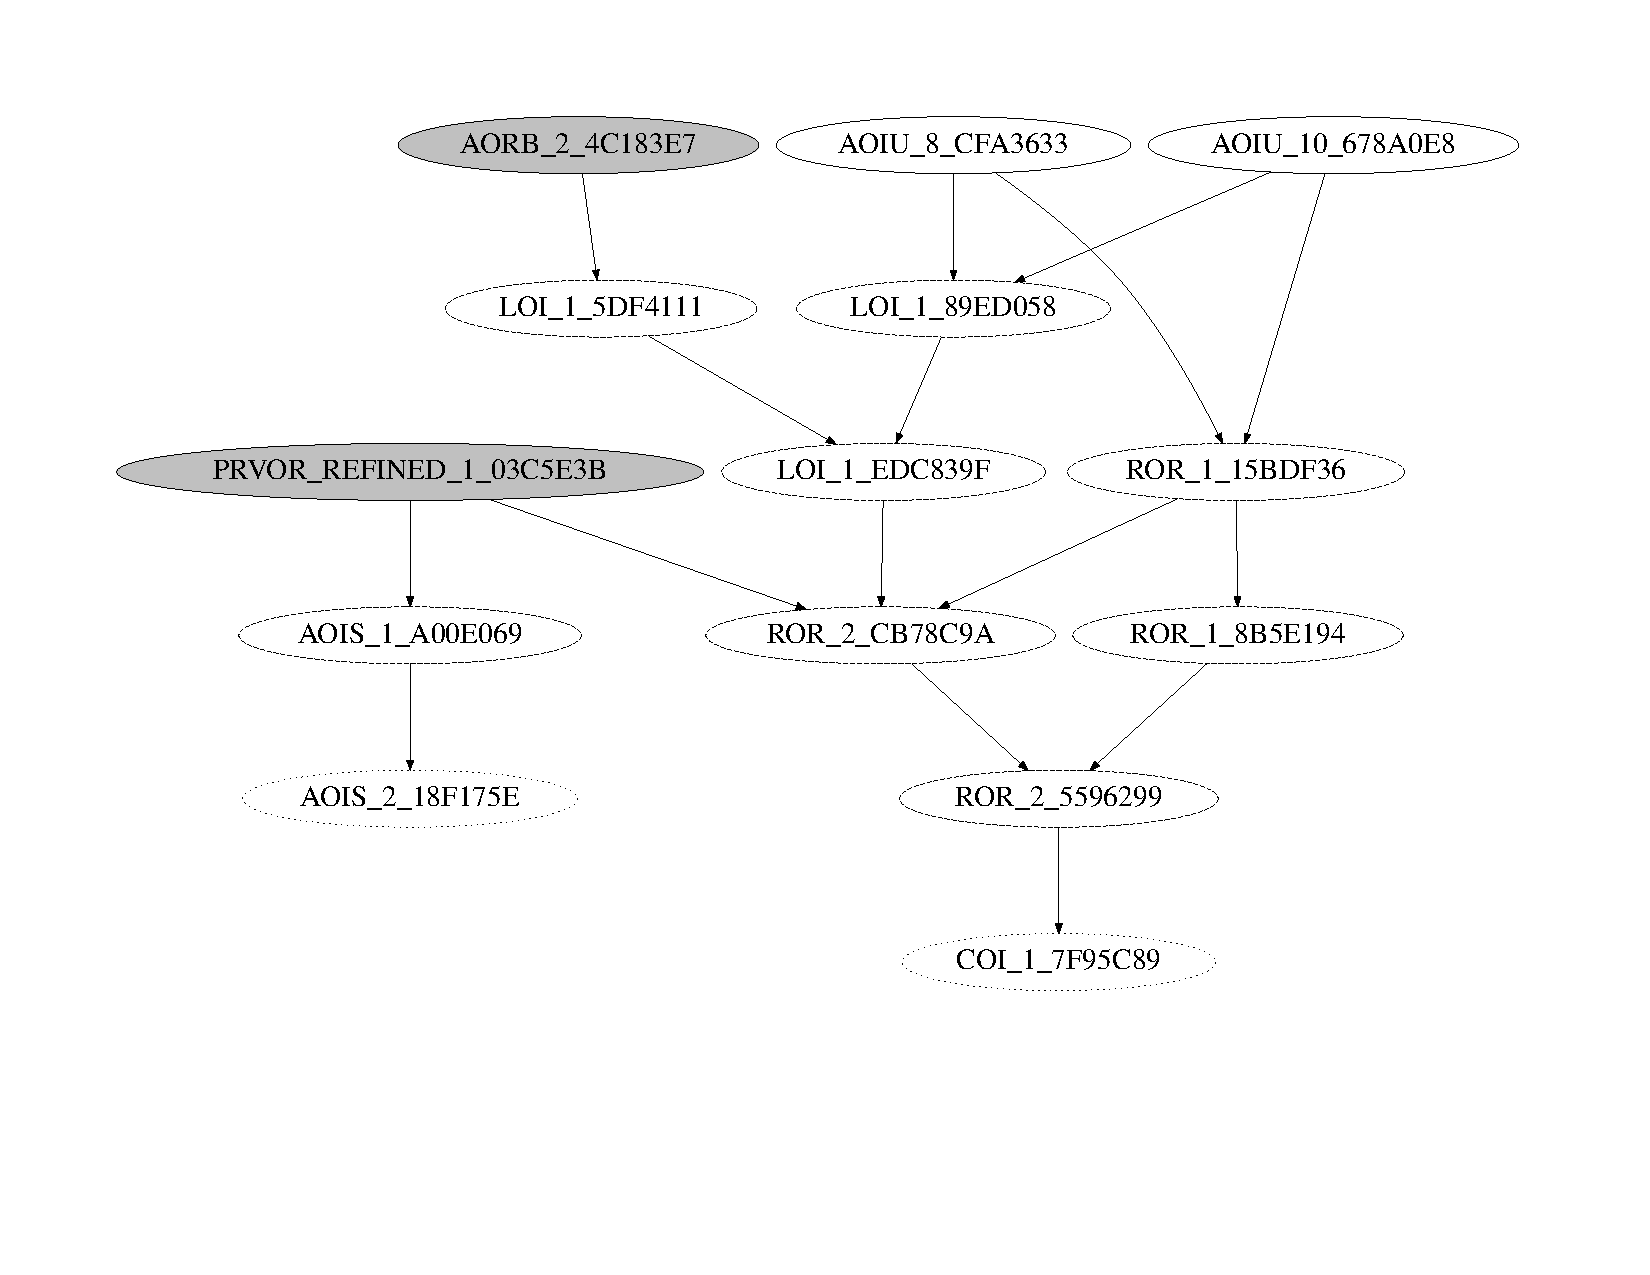
\includegraphics[width=\linewidth]{figures/subsumption/dsg_apache_prvo_segment.pdf}
	\caption[Grafo de subsunci\'on para mutantes \emph{PRVO} de \emph{TreeList}]{Grafo reducido de \emph{Dynamic Mutant Subsumption} para \emph{TreeList} con \emph{PRVO}.}
	\label{figures.examples.subsumption.reducedTreeListGraph}
\end{figure}

Las conclusiones sobre los resultados obtenidos no solamente se basan en la cantidad de nodos dominantes puros que genera \emph{PRVO}, sino tambi\'en en la relaci\'on entre los nodos dominantes donde participan los operadores suficientes con y sin la inclusi\'on de \emph{PRVO}. Principalmente, si la cantidad promedio de nodos dominantes de otros operadores aumentara al agregar \emph{PRVO}, la intuici\'on ser\'ia que \emph{PRVO} est\'a siendo subsumido. Esta situaci\'on no solo que no se observa en la mayor\'ia de los casos, sino que se observa la situaci\'on opuesta, es decir, la cantidad de nodos dominantes donde participan los operadores suficientes disminuye. Esto tomado en conjunto con el hecho de que \emph{PRVO} participa en una gran cantidad de nodos dominantes, y que a su vez suele hacerlo de manera independiente, es decir, la mayor\'ia de los nodos dominantes donde participa son puros, lleva a considerar que \emph{PRVO} estar\'ia dominando a los mutantes generados por los operadores suficientes.

En general, la observaci\'on m\'as importante al analizar los resultados es que, en casi todos los casos (con la excepci\'on de \emph{NodeCachingList}), \emph{PRVO} se posiciona entre los mejores, con respecto a dominancia, incluso es uno de los mejores tres operadores dominantes, junto a operadores t\'ipicos del conjunto de \emph{suficientes}, como \emph{ROR}, \emph{LOI}, y la familia de operadores de mutaci\'on que corresponden a la inserci\'on de operadores aritm\'eticos (\emph{AOIS}, \emph{AOIU}, y \emph{AOIB}). Es tambi\'en importante de remarcar que, en presencia de \emph{PRVO}, la dominancia de otros operadores es en general reducida, y su dominancia sobre ciertos nodos es ``transferida'' hacia \emph{PRVO}. M\'as precisamente, \emph{PRVO} domina sobre ciertos mutantes previamente (en ausencia de \emph{PRVO}) dominantes.

Un an\'alisis m\'as profundo de los resultados obtenidos con respecto a mutantes dominantes, nos lleva a dividir a \'estos en tres conjuntos. Para \emph{AvlTree}, \emph{Queue}, y \emph{BSTree}, al agregar \emph{PRVO} se obtiene una gran cantidad de nodos dominantes puros al tiempo que los nodos dominantes donde participan los operadores suficientes disminuye de manera considerable. En estos casos la participaci\'on en nodos dominantes por parte de los otros operadores llega a disminuir en algunos casos a la mitad. Para \emph{TreeList} y \emph{BinomialHeap} la dominancia de \emph{PRVO} sobre los operadores suficientes es menos notable, incluso viendo algunos casos donde la participaci\'on en nodos dominantes por parte de operadores, como \emph{AOIS}, incrementa. Finalmente el peor caso para \emph{PRVO} es \emph{NodeCachingList} donde salvo para los operadores \emph{COI} y \emph{AORS}, la participaci\'on en nodos dominantes por parte de los operadores suficientes incrementa. Sin embargo, en todos los casos \emph{PRVO} da a lugar a nodos dominantes puros, lo que indica que nunca llega a ser redundante.

Claramente, nuestros resultados experimentales resultan en una respuesta positiva a \textbf{RQ1}: \emph{PRVO} complementa de manera significativa al conjunto de operadores tradicionales; los mutantes producidos son en general no dominados por operadores existentes, y exhibe un alto n\'umero de mutantes dominantes, lo que nos permitir\'ia considerar, al menos en el contexto de nuestros experimentos, a \emph{PRVO} como un operador ``suficiente'', junto al conjunto de operadores suficientes tradicionales.

\begin{figure}[t]
	\begin{center}
		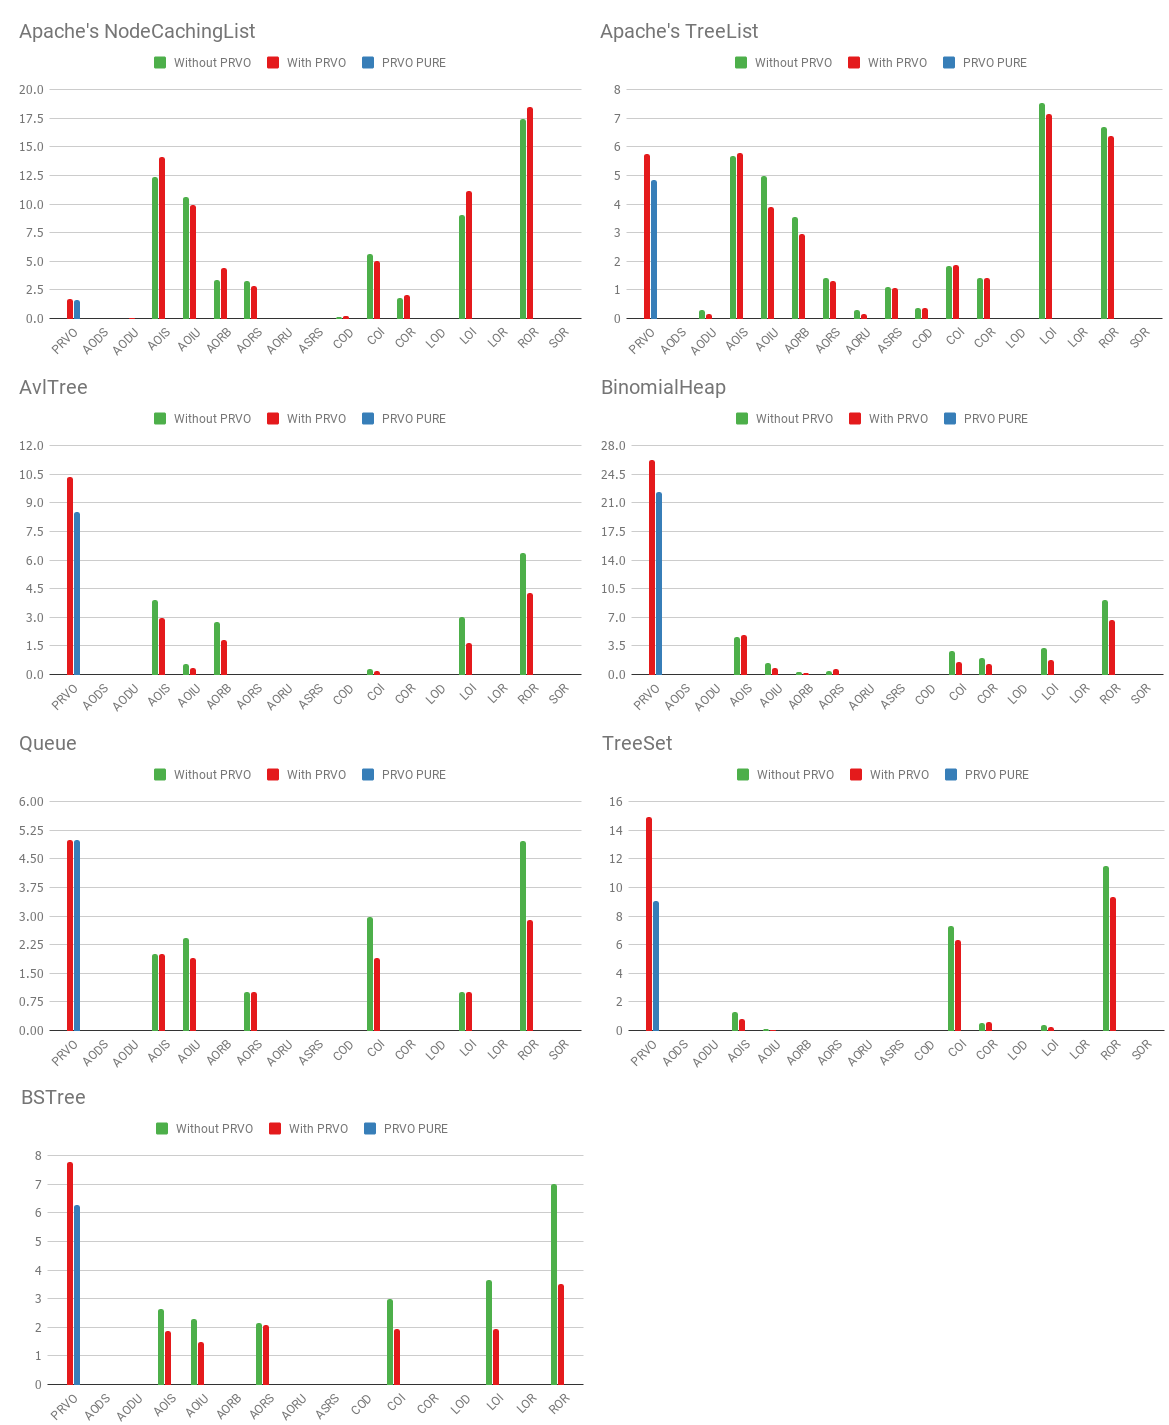
\includegraphics[width=12cm]{figures/Tables.png}
	\end{center}
	\caption{Resultados del an\'alsis de \emph{dynamic subsumption analysis}}
	\label{subsumption-results}
\end{figure}

Analicemos ahora \textbf{RQ2}. La Figura~\ref{mutants-results} y la Tabla \ref{tables.results.equivalents} resumen los resultados para generaci\'on de mutantes, comparando el n\'umero de mutantes obtenidos cuando \emph{PRVO} no es inclu\'ido (barras verdes), con los casos en donde \emph{PRVO} es considerado (barras azules). Reportamos tambi\'en, el n\'umero de mutantes equivalentes de \emph{PRVO} (mutantes que son sem\'anticamente equivalentes al programa original, y por lo tanto imposibles de detectar con cualquier test) producidos para cada caso de estudio.

Para la mayor\'ia de los casos de estudio, el n\'umero de mutantes que genera \emph{PRVO} representa solo un peque\~no incremento sobre la cantidad de mutantes generados por los operadores tradicionales. Los casos de estudio \emph{TreeSet} y \emph{BinomialHeap} son dos excepciones, en donde la cantidad de mutantes generados por \emph{PRVO} representa pr\'acticamente la misma que la generada por todos los operadores tradicionales por si solos. La raz\'on es que estos casos de estudios se caracterizan por una gran cantidad de m\'etodos, que a su vez contienen una gran cantidad de expresiones de navegaci\'on en condiciones y otras comparaciones, del tipo \texttt{expr == null}. Estas expresiones admiten una sola mutaci\'on de parte de \emph{ROR} (reemplazar el igual por un distinto), pero en donde \emph{PRVO} produce muchas mutaciones. Sin embargo, en estos dos estudios, hay que notar que \emph{PRVO} es claramente dominante (como se ve en la Figura~\ref{subsumption-results}); en particular, es notable como la dominancia de otros operadores es disminu\'ida significativamente cuando \emph{PRVO} es utilizado. Nuestra respuesta entonces para \textbf{RQ2}, es que el costo adicional, con respecto a cantidad de mutantes, de utilizar \emph{PRVO}, es en general bajo, aunque existen casos en donde el n\'umero de mutaciones generadas por \emph{PRVO} puede ``explotar''. Estos casos muestran, en nuestros experimentos, una gran dominancia por parte de \emph{PRVO} sobre mutaciones producidas por otros operadores, sugiriendo que existe un margen para realizar optimizaciones mediante priorizaci\'on de tests/mutantes, una t\'ecnica que consiste en ordenar y/o seleccionar tests o mutantes para ser evaluados antes, o en lugar, de otros, para as\'i disminuir los recursos necesarios. De todas formas, estos resultados sugieren realizar refinamientos a \emph{PRVO}, ya sea a\~nadiendo an\'alisis durante la generaci\'on de mutaciones, o implementando nuevas propiedades para configurar a \emph{PRVO} de manera m\'as apropiada para cada caso. Esto, puede llevar a lograr una mejor eficiencia, es decir una menor cantidad de mutantes, por parte de \emph{PRVO}.

Con respecto a mutantes equivalentes, los resultados son muy interesantes. La cantidad de mutantes equivalentes producidos por \emph{PRVO} fue muy poca. Esto, es muy importante, dado que cuando un operador produce muchos mutantes equivalentes: mutantes para los cuales no existe ning\'un escenario o entrada para el cual \'este se comporte de manera diferente al programa original, lo que lo hace imposible de detectar; el valor de mutation score correspondiente disminuye de manera artificial, resultando en una evaluaci\'on enga\~nosa del test suite. Tener entonces una peque\~na cantidad de dichos mutantes es un buen resultado para \emph{PRVO}. Vale la pena aclarar que si bien lo deseable es evitar por completo la generaci\'on de mutantes equivalentes, esto es en general imposible, principalmente por que al ser un problema indecidible (el detectar si un programa es equivalente a otro), no es posible tener una implementaci\'on de una herramienta de mutaci\'on que evite por completo la generaci\'on de los mismos.

El an\'alisis de \emph{Dynamic Mutant Subsumption} representa un estudio m\'as profundo que permite analizar informaci\'on que suele estar oculta cuando solo se calcula mutation score. El hecho de que \emph{PRVO} domine con respecto a este an\'alisis significa que se generan mutantes que son detectados, por lo tanto el mutation score no deber\'ia disminuir. De la misma forma, la dominancia por parte de \emph{PRVO} no es compatible con una disminuci\'on de la ``dureza'' promedio para detectar a los mutantes. Esto es confirmado por los resultados obtenidos de \emph{Mutation Score} \ref{mutationscore-results}, \emph{Toughness} \ref{toughness-results}, y \emph{Toughness de solo detectados} \ref{toughnessKilled-results}, que se condicen con los resultados de dominancia y mutantes equivalentes generados por \emph{PRVO}. El mutation score al utilizar \emph{PRVO} (en color rojo) se mantiene en general levemente por encima del obtenido al utilizar solamente los operadores suficientes (en color verde), esto junto a los resultados de dominancia, indica que la cantidad de mutantes triviales generados por \emph{PRVO} es poca (lo que llevar\'ia a un aumento del mutation score), y que la generaci\'on de mutantes equivalentes tambi\'en lo es, dado que \'estos llevar\'ian a una disminuci\'on del valor de mutation score obtenido.

Los resultados de \emph{Toughness}, tanto si se consideran todos los mutantes o solo se consideran aquellos que fueron detectados, apoyan la conclusi\'on anterior de que \emph{PRVO} no solo que no genera mutantes triviales, sino que adem\'as, \'estos son en general dif\'iciles de matar. La utilizaci\'on de test suites conformadas por una gran cantidad de tests con mayormente una cobertura de ramas alta \ref{testsAndCov-results} (lo que podr\'ia llevar a considerar a \'estas como ``suficientemente buenas'') permitir\'ia considerar como stubborn a los mutantes de \emph{PRVO} que sobrevivieron y no fueron determinados como equivalentes.

\begin{table}[]
	\caption[Casos de estudio, tests y cobertura de ramas]{Cantidad promedio de tests y cobertura de ramas para cada caso de estudio.}
	\label{testsAndCov-results}
	\centering
	\footnotesize
	\def\arraystretch{1.1}
	\setlength\tabcolsep{0.9mm}
	\begin{tabular}{|c|c|c|c|c|c|c|c|c|}
		\hline
		Project & TreeList & AvlTree & BinHeap & Queue & TreeSet & NCLL & BSTree & OrdSet\\ \cline{1-1}
		Tests & 2310 & 3391 & 3274 & 3307 & 3452 & 3819 & 3178 & 3601\\ \cline{1-1}
		Branch Cov & 100\% & 100\% & 90.3\% & 87\% & 89.46\% & 96.56\% & 94\% & 91.1\%\\ \hline
	\end{tabular}
\end{table}

\begin{figure}
	\begin{center}
		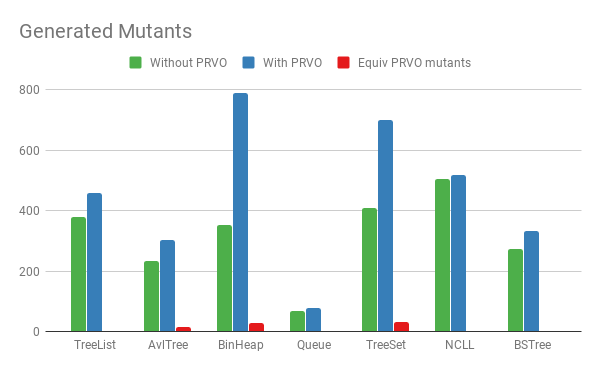
\includegraphics[width=9cm]{figures/Generated_Mutants.png}
	\end{center}
	\caption{Comparaci\'on de mutantes generados.}
	\label{mutants-results}
\end{figure}


\begin{figure}
	\begin{center}
		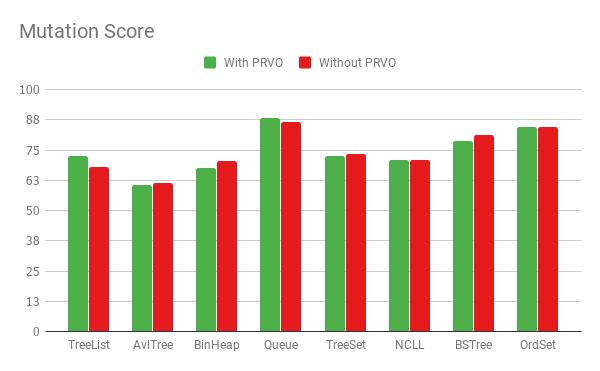
\includegraphics[width=9cm]{figures/MutationScore.png}
	\end{center}
	\caption{Comparaci\'on de \emph{Mutation score}.}
	\label{mutationscore-results}
\end{figure}

\begin{figure}
	\begin{center}
		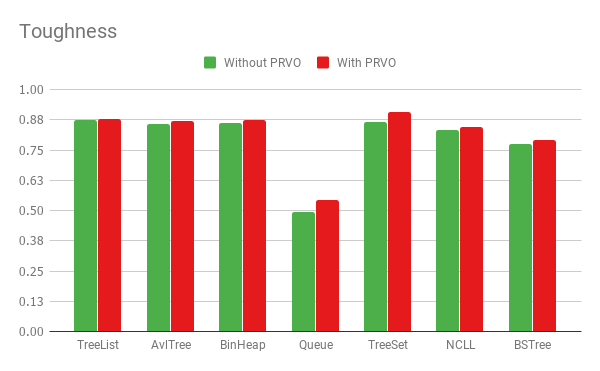
\includegraphics[width=9cm]{figures/Toughness.png}
	\end{center}
	\caption[Comparaci\'on de \emph{Toughness}]{Comparaci\'on de \emph{Toughness}, cuantos tests ``resiste'' un mutante para ser detectado, un valor de $1.0$ representa un mutante no detectado.}
	\label{toughness-results}
\end{figure}

\begin{figure}
	\begin{center}
		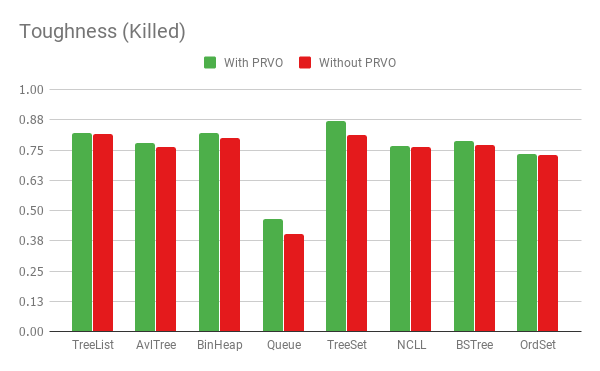
\includegraphics[width=9cm]{figures/ToughnessKilled.png}
	\end{center}
	\caption[Comparaci\'on de \emph{Toughness Killed}]{Comparaci\'on de \emph{Toughness Killed}, cuantos tests ``resiste'' un mutante que fue detectado.}
	\label{toughnessKilled-results}
\end{figure}


\section{Amenazas a la validez}

Nuestra evaluaci\'on experimental est\'a limitada a implementaciones relativamente peque\~nas de colecciones en \emph{Java}. Las razones por las que seleccionamos estas implementaciones como casos de estudio fueron parcialmente descriptas anteriormente, y esencialmente tiene que ver con que estos proyectos son buenos representantes de implementaciones orientadas a objetos con usos sofisticados de expresiones de navegaci\'on (por ejemplo, utilizan tipos de datos recursivos, y m\'ultiples referencias a objetos distintos del mismo tipo). Otra raz\'on por la que nos limitamos a estos casos de estudio tiene que ver con el alto costo de an\'alisis de mutaci\'on. Especialmente en nuestro contexto, en donde las caracter\'isticas de nuestra evaluaci\'on nos lleva a la necesidad de realizar numerosos an\'alisis de mutaci\'on, en particular, computar los grafos de subsunci\'on de mutantes har\'ia inviable esta evaluaci\'on si fu\'eramos a utilizar proyectos m\'as grandes.

Nuestro an\'alisis est\'a tambi\'en atado a una forma espec\'ifica de generar tests, \'esta se basa en el uso de dos herramientas particulares, Evosuite y Randoop espec\'ificamente. Esto est\'a motivado por el tipo de test suites que resultan de relevancia para an\'alisis de dynamic mutant subsumption. Dado el impacto que tiene el presupuesto de tiempo que se brinda a las herramientas que utilizamos para generar las test suites, nuestros resultados podr\'ian estar siendo afectados por el mismo. Para contrarrestar esta potencial amenaza, corrimos los experimentos con distintos presupuestos de tiempo, lo que llev\'o a test suites de distintos tama\~nos, pero sin embargo no obtuvimos resultados diferentes. El costo de tiempo llev\'o a realizar esta evaluaci\'on previa en un subconjunto de los casos de estudio.

La mayor parte de nuestra evaluaci\'on experimental es objetiva, es decir, provienen de an\'alisis algor\'itmicos  que retornan un valor particular, por ejemplo la noci\'on de dynamic mutant subsumption y la cantidad de mutantes generados, \'estas est\'an calculadas por nuestra implementaci\'on de \emph{$\mu$Java++} o por los scripts utilizados para automatizar los experimentos. Hicimos nuestro mejor esfuerzo para garantizar la validez de nuestros resultados, pero a\'un as\'i nuestra implementaci\'on podr\'ia contener defectos que afecten a nuestros resultados. En contraposici\'on, la equivalencia de programas, requerida para analizar mutantes equivalentes, es un problema indecidible. Varias t\'ecnicas han sido propuestas para resolver este problema (obviamente de manera aproximada), sin embargo, la verificaci\'on manual sigue siendo una de las m\'as utilizada en la pr\'actica, y es la que hemos utilizados nosotros. Afortunadamente este an\'alisis estuvo limitado a un n\'umero muy peque\~no de mutantes y cualquier duda sobre la equivalencia de uno, fue siempre anotada en desventaja de \emph{PRVO}, es decir, ante la duda, se consider\'o el mutante como equivalente. Creemos que los errores que podemos haber cometido con respecto a equivalencia de mutantes, no afectan de manera significativa nuestras conclusiones.

Nuestro an\'alisis est\'a tambi\'en limitado a un conjunto arbitrario de operadores de mutaci\'on. Podr\'iamos haber considerado otros operadores, por ejemplo los que act\'uan a nivel de clases (en contraposici\'on de los que usamos que act\'uan a nivel de m\'etodos) \cite{bibliography.mutation.class-level-ops}. \'Estos, est\'an relacionados a nuestro trabajo, en el sentido de que se aplican a programas orientados a objetos, pero se enfocan en aspectos ortogonales como visibilidad (cambiando la visibilidad de m\'etodos y campos en una clase). Decidimos concentrarnos en los operadores que se consideran tradicionales, en el contexto de mutation testing, y creemos que hemos tenido en cuenta a los m\'as significativos, basado en los que est\'an disponibles en las herramientas de mutation testing, y en estudios de operadores suficientes.

%Finalmente necesitamos remarcar que la relaci\'on de subsunci\'on de operadores, no es lo mismo que la subsunci\'on de mutantes. El primero es una relaci\'on entre operadores que es independiente de que programa se est\'e mutando, se trata de una relaci\'on que o bien se explica por la misma definici\'on de los operadores, o bien (como sucede en la mayor\'ia de los casos) requiere numerosos experimentos para determinar si es posible concluir si un operador subsume a otro. Sin embargo nuestra evaluaci\'on de subsuma din\'amica de mutantes, permite, de manera indirecta, una evaluaci\'on de la primera.

\begin{table}[]
	\caption{Mutantes generados por caso de estudio}
	\label{tables.results.mutants}
	\centering
	\footnotesize
	\def\arraystretch{1.1}
	\setlength\tabcolsep{1.0mm}
	\begin{tabular}{l|cccccccc|}
		\cline{2-9}
		& \multicolumn{1}{l}{TreeList} & \multicolumn{1}{l}{AvlTree} & \multicolumn{1}{l}{BinHeap} & \multicolumn{1}{l}{Queue} & \multicolumn{1}{l}{TreeSet} & \multicolumn{1}{l}{NCLL} & \multicolumn{1}{l}{BSTree} & \multicolumn{1}{l|}{OrdSet} \\ \hline
		\multicolumn{1}{|l|}{Sin PRVO} & 380 & 233 & 352 & 68 & 410 & 504 & 274 & 1208\\ \cline{1-1}
		\multicolumn{1}{|l|}{Con PRVO} & 458 & 304 & 788 & 78 & 700 & 519 & 334 & 1296\\ \hline
	\end{tabular}
\end{table}

\begin{table}[]
	\caption{Mutantes \emph{PRVO} equivalentes por caso de estudio}
	\label{tables.results.equivalents}
	\centering
	\footnotesize
	\def\arraystretch{1.1}
	\setlength\tabcolsep{0.5mm}
	\begin{tabular}{l|cccccccc|}
		\cline{2-9}
		& \multicolumn{1}{l}{TreeList} & \multicolumn{1}{l}{AvlTree} & \multicolumn{1}{l}{BinHeap} & \multicolumn{1}{l}{Queue} & \multicolumn{1}{l}{TreeSet} & \multicolumn{1}{l}{NCLL} &
		\multicolumn{1}{l}{BSTree} & \multicolumn{1}{l|}{OrdSet}\\ \hline
		\multicolumn{1}{|l|}{Mutantes totales} & 78 & 71 & 436 & 10 & 290 & 15 & 60 & 88\\ \cline{1-1}
		\multicolumn{1}{|l|}{Equivalentes} & 2 & 14 & 27 & 0 & 31 & 2 & 2 & 9\\ \hline
	\end{tabular}
\end{table}

\begin{table}[]
	\caption[\emph{Dynamic Mutant Subsumption} \emph{TreeList}, sin \emph{PRVO}]{Resultados de \emph{Dynamic Mutant Subsumption} para \emph{TreeList}, sin \emph{PRVO}}
	\label{tables.results.subsumption.treelist.noprvo}
	\centering
	\scriptsize
	\def\arraystretch{0.95}
	\setlength\tabcolsep{0.5mm}
	\begin{tabular}{rrrrrrrrrrrrr}
		DOM NODES & AODU & AOIS & AOIU & AORB & AORS & AORU & ASRS & COD & COI & COR & LOI & ROR \\
		24 & 0 & 10 & 3 & 4 & 2 & 0 & 1 & 0 & 1 & 1 & 8 & 6 \\
		23 & 0 & 8 & 4 & 2 & 1 & 0 & 0 & 0 & 2 & 1 & 7 & 5 \\
		21 & 0 & 4 & 4 & 3 & 1 & 0 & 1 & 1 & 3 & 2 & 9 & 7 \\
		16 & 0 & 5 & 2 & 3 & 1 & 0 & 1 & 1 & 1 & 0 & 8 & 5 \\
		21 & 0 & 5 & 7 & 5 & 1 & 0 & 1 & 1 & 3 & 2 & 7 & 7 \\
		23 & 0 & 8 & 6 & 4 & 2 & 0 & 1 & 1 & 3 & 3 & 11 & 6 \\
		23 & 0 & 4 & 7 & 2 & 1 & 0 & 2 & 1 & 3 & 2 & 9 & 7 \\
		23 & 0 & 6 & 4 & 3 & 2 & 0 & 1 & 1 & 3 & 3 & 10 & 7 \\
		26 & 0 & 8 & 2 & 3 & 0 & 0 & 1 & 0 & 1 & 0 & 8 & 7 \\
		22 & 0 & 6 & 6 & 3 & 2 & 0 & 1 & 0 & 3 & 1 & 8 & 7 \\
		15 & 1 & 5 & 6 & 3 & 2 & 1 & 0 & 0 & 4 & 2 & 7 & 8 \\
		27 & 0 & 7 & 4 & 4 & 2 & 0 & 2 & 1 & 3 & 3 & 8 & 9 \\
		19 & 0 & 4 & 5 & 4 & 1 & 0 & 1 & 1 & 3 & 3 & 9 & 7 \\
		19 & 1 & 5 & 6 & 5 & 1 & 1 & 1 & 0 & 4 & 2 & 8 & 8 \\
		24 & 0 & 8 & 5 & 4 & 1 & 0 & 0 & 0 & 2 & 1 & 8 & 7 \\
		21 & 0 & 5 & 8 & 4 & 1 & 0 & 2 & 1 & 1 & 3 & 8 & 7 \\
		23 & 1 & 7 & 5 & 2 & 1 & 1 & 1 & 0 & 2 & 0 & 6 & 7 \\
		25 & 1 & 6 & 4 & 4 & 0 & 1 & 1 & 0 & 3 & 2 & 9 & 10 \\
		22 & 0 & 6 & 4 & 2 & 1 & 0 & 3 & 1 & 2 & 1 & 8 & 6 \\
		19 & 0 & 6 & 4 & 3 & 1 & 0 & 2 & 1 & 1 & 2 & 8 & 4 \\
		26 & 0 & 4 & 5 & 2 & 2 & 0 & 1 & 0 & 2 & 2 & 7 & 9 \\
		23 & 0 & 6 & 6 & 3 & 0 & 0 & 2 & 0 & 1 & 1 & 6 & 9 \\
		17 & 0 & 1 & 5 & 4 & 0 & 0 & 0 & 0 & 1 & 2 & 4 & 7 \\
		26 & 1 & 6 & 4 & 2 & 0 & 1 & 0 & 0 & 3 & 2 & 6 & 11 \\
		23 & 0 & 7 & 6 & 4 & 1 & 0 & 2 & 0 & 2 & 1 & 7 & 6 \\
		20 & 0 & 7 & 3 & 2 & 0 & 0 & 2 & 0 & 0 & 0 & 9 & 7 \\
		21 & 1 & 2 & 7 & 4 & 1 & 1 & 1 & 1 & 3 & 2 & 7 & 9 \\
		22 & 0 & 4 & 5 & 5 & 2 & 0 & 3 & 0 & 0 & 0 & 7 & 6 \\
		24 & 0 & 8 & 3 & 3 & 1 & 0 & 1 & 0 & 2 & 1 & 8 & 7 \\
		22 & 0 & 6 & 5 & 4 & 2 & 0 & 1 & 0 & 2 & 0 & 8 & 4
	\end{tabular}
\end{table}

\begin{table}[]
	\caption[\emph{Dynamic Mutant Subsumption} \emph{TreeList}, con \emph{PRVO}]{Resultados de \emph{Dynamic Mutant Subsumption} para \emph{TreeList}, con \emph{PRVO}}
	\label{tables.results.subsumption.treelist.prvo}
	\centering
	\scriptsize
	\def\arraystretch{0.95}
	\setlength\tabcolsep{0.5mm}
	\begin{tabular}{rrrrrrrrrrrrrr}
		DOM NODES & PRVO & AODU & AOIS & AOIU & AORB & AORS & AORU & ASRS & COD & COI & COR & LOI & ROR \\
		15 & 4 & 1 & 5 & 6 & 3 & 2 & 1 & 0 & 0 & 4 & 2 & 7 & 8 \\
		22 & 4 & 0 & 4 & 5 & 4 & 1 & 0 & 1 & 1 & 3 & 3 & 9 & 7 \\
		30 & 8 & 0 & 8 & 3 & 4 & 1 & 0 & 0 & 0 & 2 & 1 & 7 & 7 \\
		22 & 4 & 0 & 3 & 7 & 4 & 1 & 0 & 2 & 1 & 1 & 3 & 7 & 7 \\
		21 & 6 & 0 & 4 & 3 & 3 & 1 & 0 & 1 & 1 & 2 & 2 & 7 & 6 \\
		24 & 7 & 0 & 4 & 7 & 2 & 1 & 0 & 2 & 1 & 3 & 2 & 8 & 6 \\
		27 & 6 & 0 & 6 & 6 & 3 & 2 & 0 & 1 & 0 & 3 & 1 & 8 & 7 \\
		33 & 8 & 0 & 8 & 2 & 3 & 0 & 0 & 1 & 0 & 1 & 0 & 8 & 7 \\
		28 & 8 & 1 & 3 & 3 & 3 & 0 & 1 & 1 & 0 & 2 & 1 & 7 & 9 \\
		24 & 6 & 1 & 2 & 7 & 4 & 1 & 1 & 1 & 1 & 2 & 2 & 7 & 7 \\
		20 & 2 & 1 & 5 & 6 & 5 & 1 & 1 & 1 & 0 & 4 & 2 & 8 & 8 \\
		29 & 7 & 0 & 6 & 5 & 3 & 0 & 0 & 2 & 0 & 1 & 1 & 6 & 9 \\
		28 & 4 & 0 & 8 & 3 & 3 & 1 & 0 & 1 & 0 & 2 & 1 & 8 & 7 \\
		26 & 5 & 0 & 7 & 4 & 4 & 1 & 0 & 2 & 0 & 2 & 1 & 7 & 6 \\
		27 & 5 & 0 & 8 & 4 & 2 & 1 & 0 & 0 & 0 & 2 & 1 & 7 & 5 \\
		35 & 10 & 1 & 6 & 3 & 2 & 0 & 1 & 0 & 0 & 3 & 2 & 6 & 11 \\
		24 & 9 & 0 & 5 & 1 & 3 & 1 & 0 & 1 & 1 & 1 & 0 & 8 & 5 \\
		23 & 8 & 0 & 1 & 3 & 3 & 0 & 0 & 0 & 0 & 1 & 2 & 4 & 7 \\
		32 & 7 & 0 & 7 & 3 & 3 & 2 & 0 & 2 & 1 & 3 & 3 & 8 & 9 \\
		22 & 4 & 0 & 5 & 3 & 2 & 0 & 0 & 2 & 0 & 0 & 0 & 9 & 7 \\
		22 & 5 & 0 & 5 & 3 & 3 & 2 & 0 & 1 & 1 & 3 & 3 & 7 & 6 \\
		24 & 5 & 0 & 8 & 5 & 4 & 2 & 0 & 1 & 1 & 1 & 3 & 9 & 5 \\
		25 & 5 & 0 & 4 & 4 & 4 & 2 & 0 & 3 & 0 & 0 & 0 & 7 & 6 \\
		24 & 6 & 0 & 9 & 2 & 3 & 1 & 0 & 1 & 0 & 1 & 1 & 7 & 4 \\
		27 & 5 & 0 & 6 & 4 & 2 & 1 & 0 & 3 & 1 & 2 & 1 & 8 & 6 \\
		23 & 5 & 0 & 6 & 4 & 3 & 1 & 0 & 2 & 1 & 1 & 2 & 8 & 4 \\
		31 & 6 & 0 & 4 & 5 & 2 & 2 & 0 & 1 & 0 & 2 & 2 & 7 & 9 \\
		25 & 7 & 0 & 6 & 4 & 4 & 2 & 0 & 1 & 0 & 2 & 0 & 7 & 4 \\
		25 & 5 & 0 & 5 & 6 & 5 & 1 & 0 & 1 & 1 & 3 & 2 & 6 & 7 \\
		29 & 7 & 1 & 7 & 4 & 2 & 1 & 1 & 1 & 0 & 2 & 0 & 6 & 7
	\end{tabular}
\end{table}

\begin{table}[]
	\caption[\emph{Dynamic Mutant Subsumption} \emph{AvlTree}, sin \emph{PRVO}]{Resultados de \emph{Dynamic Mutant Subsumption} para \emph{AvlTree}, sin \emph{PRVO}}
	\label{tables.results.subsumption.avltree.noprvo}
	\centering
	\scriptsize
	\def\arraystretch{0.95}
	\setlength\tabcolsep{0.5mm}
	\begin{tabular}{rrrrrrr}
		DOM NODES & AOIS & AOIU & AORB & COI & LOI & ROR \\
		13 & 2 & 0 & 3 & 1 & 3 & 6 \\
		17 & 6 & 0 & 2 & 1 & 5 & 6 \\
		21 & 5 & 1 & 4 & 1 & 4 & 8 \\
		21 & 7 & 1 & 4 & 1 & 4 & 7 \\
		21 & 5 & 1 & 3 & 0 & 4 & 9 \\
		19 & 5 & 0 & 4 & 1 & 4 & 8 \\
		20 & 7 & 0 & 4 & 0 & 3 & 8 \\
		16 & 5 & 0 & 3 & 0 & 3 & 5 \\
		23 & 9 & 3 & 3 & 0 & 2 & 6 \\
		12 & 2 & 0 & 4 & 0 & 3 & 4 \\
		17 & 4 & 0 & 2 & 0 & 2 & 11 \\
		14 & 2 & 0 & 4 & 0 & 3 & 5 \\
		17 & 4 & 1 & 3 & 0 & 3 & 7 \\
		21 & 4 & 2 & 3 & 0 & 3 & 10 \\
		12 & 7 & 0 & 2 & 0 & 1 & 3 \\
		13 & 2 & 0 & 3 & 1 & 3 & 6 \\
		23 & 6 & 2 & 4 & 0 & 5 & 7 \\
		13 & 4 & 0 & 4 & 0 & 2 & 4 \\
		21 & 7 & 1 & 3 & 0 & 5 & 7 \\
		19 & 4 & 1 & 4 & 0 & 4 & 7 \\
		21 & 7 & 1 & 4 & 1 & 2 & 8 \\
		21 & 6 & 0 & 4 & 0 & 4 & 9 \\
		19 & 7 & 1 & 3 & 1 & 3 & 7 \\
		22 & 7 & 1 & 2 & 0 & 6 & 8 \\
		13 & 2 & 1 & 3 & 1 & 4 & 5 \\
		15 & 5 & 0 & 2 & 0 & 4 & 6 \\
		17 & 3 & 1 & 3 & 0 & 5 & 7 \\
		11 & 2 & 0 & 3 & 0 & 3 & 4 \\
		17 & 4 & 1 & 3 & 1 & 4 & 6 \\
		22 & 8 & 1 & 3 & 0 & 4 & 7
	\end{tabular}
\end{table}

\begin{table}[]
	\caption[\emph{Dynamic Mutant Subsumption} \emph{AvlTree}, con \emph{PRVO}]{Resultados de \emph{Dynamic Mutant Subsumption} para \emph{AvlTree}, con \emph{PRVO}}
	\label{tables.results.subsumption.avltree.prvo}
	\centering
	\scriptsize
	\def\arraystretch{0.95}
	\setlength\tabcolsep{0.5mm}
	\begin{tabular}{rrrrrrrr}
		DOM NODES & PRVO & AOIS & AOIU & AORB & COI & LOI & ROR \\
		23 & 9 & 5 & 1 & 2 & 0 & 2 & 5 \\
		18 & 8 & 2 & 0 & 3 & 0 & 1 & 5 \\
		19 & 8 & 3 & 1 & 1 & 0 & 4 & 4 \\
		21 & 10 & 3 & 1 & 2 & 0 & 2 & 5 \\
		19 & 11 & 2 & 0 & 4 & 0 & 1 & 3 \\
		19 & 9 & 2 & 0 & 3 & 0 & 1 & 4 \\
		20 & 12 & 3 & 0 & 2 & 0 & 1 & 4 \\
		21 & 4 & 5 & 2 & 3 & 0 & 2 & 6 \\
		25 & 15 & 5 & 0 & 1 & 0 & 2 & 4 \\
		21 & 11 & 4 & 0 & 2 & 1 & 2 & 5 \\
		21 & 13 & 4 & 0 & 0 & 0 & 0 & 6 \\
		25 & 10 & 4 & 2 & 3 & 0 & 1 & 7 \\
		21 & 10 & 6 & 1 & 2 & 0 & 1 & 3 \\
		16 & 7 & 4 & 0 & 2 & 0 & 1 & 4 \\
		26 & 13 & 5 & 1 & 3 & 0 & 1 & 5 \\
		30 & 15 & 5 & 1 & 4 & 0 & 1 & 6 \\
		27 & 14 & 4 & 1 & 3 & 0 & 1 & 6 \\
		15 & 7 & 2 & 1 & 3 & 0 & 1 & 2 \\
		21 & 9 & 5 & 0 & 3 & 0 & 2 & 5 \\
		22 & 11 & 7 & 0 & 2 & 0 & 1 & 3 \\
		15 & 10 & 2 & 0 & 2 & 0 & 0 & 2 \\
		19 & 11 & 2 & 0 & 1 & 1 & 3 & 5 \\
		22 & 11 & 3 & 2 & 3 & 0 & 1 & 3 \\
		16 & 6 & 3 & 0 & 3 & 0 & 1 & 3 \\
		27 & 13 & 5 & 1 & 4 & 0 & 2 & 4 \\
		13 & 6 & 2 & 0 & 3 & 0 & 1 & 1 \\
		22 & 8 & 3 & 1 & 2 & 1 & 4 & 6 \\
		14 & 5 & 2 & 0 & 3 & 0 & 1 & 3 \\
		18 & 8 & 4 & 0 & 4 & 0 & 1 & 2 \\
		24 & 12 & 5 & 1 & 3 & 1 & 2 & 5
	\end{tabular}
\end{table}

\begin{table}[]
	\caption[\emph{Dynamic Mutant Subsumption} \emph{Binheap}, sin \emph{PRVO}]{Resultados de \emph{Dynamic Mutant Subsumption} para \emph{Binheap}, sin \emph{PRVO}}
	\label{tables.results.subsumption.binheap.noprvo}
	\centering
	\scriptsize
	\def\arraystretch{0.95}
	\setlength\tabcolsep{0.5mm}
	\begin{tabular}{rrrrrrrrr}
		DOM NODES & AOIS & AOIU & AORB & AORS & COI & COR & LOI & ROR \\
		17 & 8 & 1 & 0 & 0 & 4 & 2 & 5 & 12 \\
		9 & 5 & 0 & 0 & 1 & 2 & 2 & 1 & 6 \\
		15 & 6 & 2 & 0 & 0 & 1 & 1 & 3 & 8 \\
		18 & 6 & 1 & 0 & 1 & 4 & 3 & 7 & 14 \\
		12 & 6 & 1 & 0 & 2 & 3 & 2 & 4 & 9 \\
		19 & 7 & 2 & 1 & 1 & 2 & 2 & 3 & 9 \\
		15 & 5 & 1 & 1 & 1 & 3 & 3 & 6 & 10 \\
		15 & 9 & 2 & 0 & 1 & 1 & 0 & 3 & 6 \\
		18 & 7 & 3 & 0 & 0 & 3 & 3 & 6 & 12 \\
		19 & 6 & 1 & 1 & 1 & 4 & 3 & 5 & 12 \\
		13 & 5 & 1 & 0 & 1 & 4 & 2 & 3 & 11 \\
		13 & 7 & 1 & 1 & 0 & 2 & 2 & 2 & 8 \\
		9 & 5 & 0 & 0 & 0 & 2 & 1 & 2 & 4 \\
		15 & 8 & 1 & 0 & 0 & 2 & 2 & 3 & 8 \\
		14 & 4 & 1 & 1 & 0 & 4 & 0 & 3 & 9 \\
		12 & 5 & 0 & 1 & 1 & 2 & 1 & 2 & 8 \\
		14 & 6 & 2 & 1 & 0 & 3 & 3 & 5 & 11 \\
		15 & 4 & 0 & 1 & 0 & 3 & 3 & 4 & 12 \\
		17 & 6 & 2 & 0 & 0 & 2 & 4 & 4 & 13 \\
		15 & 6 & 2 & 0 & 0 & 2 & 2 & 5 & 10 \\
		8 & 3 & 1 & 0 & 0 & 2 & 2 & 2 & 7 \\
		13 & 4 & 2 & 0 & 2 & 3 & 2 & 1 & 8 \\
		21 & 7 & 2 & 0 & 2 & 4 & 3 & 4 & 13 \\
		14 & 6 & 1 & 1 & 0 & 3 & 2 & 3 & 9 \\
		13 & 3 & 2 & 0 & 1 & 3 & 2 & 1 & 8 \\
		14 & 7 & 2 & 0 & 1 & 3 & 2 & 4 & 9 \\
		9 & 4 & 0 & 0 & 0 & 3 & 2 & 3 & 7 \\
		20 & 7 & 1 & 1 & 0 & 2 & 3 & 4 & 11 \\
		11 & 6 & 2 & 1 & 1 & 2 & 1 & 4 & 6 \\
		9 & 3 & 0 & 0 & 0 & 5 & 0 & 3 & 9
	\end{tabular}
\end{table}

\begin{table}[]
	\caption[\emph{Dynamic Mutant Subsumption} \emph{Binheap}, con \emph{PRVO}]{Resultados de \emph{Dynamic Mutant Subsumption} para \emph{Binheap}, con \emph{PRVO}}
	\label{tables.results.subsumption.binheap.prvo}
	\centering
	\scriptsize
	\def\arraystretch{0.95}
	\setlength\tabcolsep{0.5mm}
	\begin{tabular}{rrrrrrrrrr}
		DOM NODES & PRVO & AOIS & AOIU & AORB & AORS & COI & COR & LOI & ROR \\
		20 & 16 & 3 & 0 & 1 & 0 & 2 & 1 & 2 & 5 \\
		16 & 14 & 4 & 0 & 0 & 1 & 2 & 1 & 1 & 4 \\
		22 & 15 & 5 & 1 & 0 & 0 & 1 & 1 & 2 & 7 \\
		20 & 18 & 5 & 1 & 1 & 1 & 1 & 1 & 3 & 4 \\
		22 & 17 & 2 & 1 & 0 & 2 & 1 & 1 & 1 & 3 \\
		19 & 14 & 5 & 1 & 1 & 0 & 1 & 1 & 1 & 5 \\
		21 & 14 & 4 & 1 & 1 & 0 & 2 & 1 & 3 & 7 \\
		20 & 14 & 4 & 0 & 1 & 1 & 1 & 0 & 2 & 5 \\
		18 & 16 & 3 & 0 & 0 & 0 & 2 & 1 & 3 & 5 \\
		19 & 15 & 2 & 0 & 1 & 0 & 2 & 0 & 1 & 4 \\
		13 & 11 & 5 & 0 & 0 & 0 & 1 & 1 & 2 & 3 \\
		29 & 22 & 4 & 1 & 0 & 2 & 2 & 2 & 2 & 8 \\
		19 & 12 & 8 & 2 & 0 & 1 & 1 & 0 & 2 & 5 \\
		20 & 15 & 7 & 0 & 0 & 0 & 1 & 1 & 2 & 5 \\
		25 & 19 & 4 & 1 & 0 & 0 & 2 & 1 & 3 & 8 \\
		16 & 11 & 3 & 1 & 0 & 2 & 3 & 1 & 2 & 6 \\
		24 & 20 & 2 & 0 & 0 & 0 & 3 & 0 & 2 & 7 \\
		21 & 15 & 3 & 1 & 1 & 1 & 2 & 1 & 5 & 7 \\
		20 & 14 & 3 & 1 & 0 & 1 & 1 & 2 & 0 & 5 \\
		28 & 22 & 6 & 2 & 0 & 0 & 0 & 2 & 2 & 6 \\
		23 & 16 & 5 & 2 & 1 & 0 & 2 & 2 & 5 & 9 \\
		14 & 12 & 3 & 0 & 0 & 0 & 2 & 0 & 3 & 4 \\
		22 & 20 & 3 & 1 & 0 & 1 & 2 & 1 & 2 & 5 \\
		18 & 15 & 2 & 1 & 0 & 0 & 1 & 1 & 1 & 4 \\
		26 & 19 & 4 & 1 & 0 & 1 & 2 & 2 & 5 & 8 \\
		21 & 16 & 4 & 1 & 0 & 0 & 2 & 2 & 3 & 7 \\
		25 & 20 & 3 & 0 & 1 & 1 & 3 & 1 & 5 & 6 \\
		25 & 18 & 4 & 1 & 1 & 1 & 1 & 1 & 1 & 4 \\
		20 & 17 & 2 & 1 & 0 & 1 & 3 & 1 & 1 & 4 \\
		25 & 21 & 5 & 0 & 1 & 0 & 1 & 1 & 2 & 4
	\end{tabular}
\end{table}

\begin{table}[]
	\caption[\emph{Dynamic Mutant Subsumption} \emph{TreeSet}, sin \emph{PRVO}]{Resultados de \emph{Dynamic Mutant Subsumption} para \emph{TreeSet}, sin \emph{PRVO}}
	\label{tables.results.subsumption.treeset.noprvo}
	\centering
	\scriptsize
	\def\arraystretch{0.95}
	\setlength\tabcolsep{0.5mm}
	\begin{tabular}{rrrrrrr}
		DOM NODES & AOIS & AOIU & COI & COR & LOI & ROR \\
		13 & 1 & 1 & 8 & 1 & 1 & 11 \\
		14 & 1 & 0 & 6 & 1 & 0 & 12 \\
		9 & 1 & 0 & 4 & 1 & 0 & 8 \\
		22 & 3 & 1 & 4 & 1 & 2 & 18 \\
		18 & 2 & 1 & 7 & 0 & 2 & 13 \\
		14 & 0 & 0 & 9 & 0 & 0 & 12 \\
		14 & 2 & 0 & 7 & 1 & 1 & 11 \\
		13 & 1 & 0 & 7 & 1 & 0 & 12 \\
		18 & 2 & 0 & 7 & 1 & 1 & 13 \\
		15 & 1 & 0 & 6 & 1 & 0 & 13 \\
		15 & 0 & 1 & 10 & 2 & 1 & 14 \\
		17 & 1 & 1 & 9 & 0 & 0 & 14 \\
		13 & 1 & 0 & 8 & 1 & 0 & 10 \\
		17 & 1 & 0 & 8 & 1 & 0 & 12 \\
		23 & 3 & 0 & 10 & 0 & 1 & 18 \\
		18 & 5 & 0 & 7 & 2 & 1 & 12 \\
		23 & 3 & 0 & 10 & 1 & 1 & 16 \\
		14 & 1 & 0 & 9 & 2 & 0 & 11 \\
		14 & 1 & 0 & 10 & 1 & 0 & 7 \\
		17 & 3 & 0 & 4 & 2 & 1 & 11 \\
		15 & 1 & 1 & 5 & 1 & 1 & 13 \\
		16 & 1 & 0 & 8 & 0 & 0 & 13 \\
		15 & 1 & 0 & 9 & 0 & 0 & 11 \\
		16 & 2 & 1 & 8 & 0 & 1 & 15 \\
		15 & 0 & 0 & 8 & 0 & 0 & 13 \\
		19 & 2 & 0 & 7 & 1 & 1 & 15 \\
		16 & 2 & 1 & 9 & 0 & 1 & 11 \\
		18 & 3 & 1 & 8 & 1 & 2 & 14 \\
		14 & 0 & 0 & 10 & 1 & 0 & 10 \\
		13 & 2 & 1 & 6 & 0 & 0 & 10
	\end{tabular}
\end{table}

\begin{table}[]
	\caption[\emph{Dynamic Mutant Subsumption} \emph{TreeSet}, con \emph{PRVO}]{Resultados de \emph{Dynamic Mutant Subsumption} para \emph{TreeSet}, con \emph{PRVO}}
	\label{tables.results.subsumption.treeset.prvo}
	\centering
	\scriptsize
	\def\arraystretch{0.95}
	\setlength\tabcolsep{0.5mm}
	\begin{tabular}{rrrrrrrr}
		DOM NODES & PRVO & AOIS & AOIU & COI & COR & LOI & ROR \\
		23 & 19 & 1 & 0 & 7 & 1 & 0 & 12 \\
		22 & 14 & 0 & 1 & 7 & 0 & 1 & 10 \\
		19 & 13 & 1 & 1 & 8 & 1 & 1 & 10 \\
		22 & 14 & 3 & 0 & 6 & 2 & 1 & 10 \\
		28 & 21 & 1 & 0 & 7 & 1 & 0 & 8 \\
		26 & 20 & 0 & 0 & 8 & 0 & 0 & 8 \\
		19 & 13 & 1 & 0 & 7 & 1 & 0 & 9 \\
		21 & 12 & 2 & 0 & 3 & 2 & 1 & 10 \\
		21 & 16 & 1 & 0 & 8 & 0 & 0 & 9 \\
		18 & 16 & 0 & 0 & 5 & 1 & 0 & 9 \\
		25 & 17 & 3 & 1 & 7 & 1 & 2 & 13 \\
		19 & 15 & 2 & 0 & 4 & 0 & 0 & 6 \\
		19 & 14 & 0 & 0 & 6 & 0 & 0 & 6 \\
		16 & 13 & 1 & 0 & 4 & 1 & 0 & 8 \\
		20 & 14 & 0 & 0 & 7 & 1 & 0 & 8 \\
		19 & 14 & 1 & 0 & 8 & 2 & 0 & 7 \\
		23 & 17 & 0 & 0 & 4 & 1 & 0 & 7 \\
		27 & 22 & 1 & 0 & 6 & 1 & 0 & 11 \\
		30 & 22 & 2 & 0 & 9 & 1 & 0 & 10 \\
		24 & 19 & 1 & 0 & 8 & 1 & 0 & 4 \\
		24 & 17 & 2 & 1 & 8 & 0 & 1 & 14 \\
		20 & 15 & 0 & 1 & 8 & 2 & 1 & 10 \\
		24 & 20 & 0 & 0 & 5 & 1 & 0 & 10 \\
		28 & 22 & 1 & 0 & 7 & 0 & 0 & 10 \\
		23 & 16 & 1 & 0 & 5 & 1 & 0 & 11 \\
		20 & 13 & 1 & 1 & 8 & 0 & 0 & 8 \\
		23 & 16 & 0 & 0 & 9 & 1 & 0 & 8 \\
		25 & 21 & 0 & 0 & 7 & 0 & 0 & 9 \\
		23 & 18 & 1 & 0 & 3 & 1 & 0 & 7 \\
		23 & 15 & 2 & 1 & 7 & 0 & 1 & 10
	\end{tabular}
\end{table}

\begin{table}[]
	\caption[\emph{Dynamic Mutant Subsumption} \emph{NodeCachingList}, sin \emph{PRVO}]{Resultados de \emph{Dynamic Mutant Subsumption} para \emph{NodeCachingList}, sin \emph{PRVO}}
	\label{tables.results.subsumption.ncll.noprvo}
	\centering
	\scriptsize
	\def\arraystretch{0.95}
	\setlength\tabcolsep{0.5mm}
	\begin{tabular}{rrrrrrrrrrrr}
		DOM NODES & AODU & AOIS & AOIU & AORB & AORS & AORU & COD & COI & COR & LOI & ROR \\
		60 & 1 & 11 & 14 & 1 & 5 & 1 & 0 & 9 & 2 & 11 & 22 \\
		67 & 1 & 11 & 19 & 2 & 5 & 1 & 0 & 12 & 2 & 11 & 25 \\
		58 & 0 & 12 & 16 & 2 & 4 & 0 & 0 & 10 & 0 & 11 & 22 \\
		49 & 0 & 7 & 13 & 1 & 4 & 0 & 0 & 8 & 3 & 7 & 20 \\
		59 & 0 & 13 & 13 & 1 & 5 & 0 & 0 & 10 & 1 & 12 & 22 \\
		72 & 1 & 14 & 17 & 0 & 6 & 1 & 0 & 14 & 2 & 11 & 24 \\
		64 & 0 & 13 & 16 & 1 & 5 & 0 & 0 & 9 & 1 & 12 & 22 \\
		65 & 1 & 13 & 18 & 1 & 6 & 1 & 0 & 12 & 2 & 10 & 22 \\
		65 & 1 & 11 & 15 & 0 & 5 & 1 & 0 & 10 & 2 & 11 & 25 \\
		62 & 1 & 15 & 15 & 1 & 6 & 1 & 1 & 12 & 2 & 9 & 20 \\
		60 & 0 & 15 & 12 & 1 & 5 & 0 & 0 & 9 & 2 & 12 & 22 \\
		59 & 1 & 13 & 13 & 1 & 5 & 1 & 0 & 9 & 2 & 8 & 21 \\
		66 & 0 & 14 & 16 & 0 & 5 & 0 & 0 & 10 & 1 & 9 & 22 \\
		67 & 1 & 16 & 14 & 1 & 6 & 1 & 0 & 11 & 1 & 10 & 24 \\
		64 & 0 & 13 & 18 & 3 & 5 & 0 & 0 & 10 & 1 & 12 & 25 \\
		70 & 0 & 13 & 16 & 1 & 6 & 0 & 0 & 11 & 2 & 10 & 24 \\
		63 & 0 & 11 & 16 & 1 & 5 & 0 & 0 & 12 & 2 & 11 & 23 \\
		65 & 0 & 10 & 17 & 1 & 6 & 0 & 0 & 11 & 1 & 11 & 22 \\
		66 & 1 & 14 & 17 & 0 & 6 & 1 & 0 & 11 & 2 & 8 & 22 \\
		72 & 1 & 14 & 18 & 1 & 6 & 1 & 0 & 10 & 2 & 12 & 26 \\
		59 & 0 & 10 & 15 & 2 & 6 & 0 & 0 & 11 & 1 & 12 & 21 \\
		64 & 1 & 14 & 16 & 1 & 6 & 1 & 0 & 11 & 2 & 8 & 23 \\
		64 & 1 & 15 & 16 & 2 & 5 & 1 & 0 & 11 & 2 & 10 & 23 \\
		58 & 1 & 13 & 15 & 1 & 3 & 1 & 0 & 7 & 2 & 10 & 20 \\
		57 & 1 & 10 & 13 & 1 & 4 & 1 & 0 & 10 & 2 & 7 & 24 \\
		58 & 1 & 15 & 12 & 1 & 3 & 1 & 0 & 11 & 1 & 10 & 22 \\
		61 & 0 & 10 & 18 & 1 & 4 & 0 & 0 & 10 & 1 & 9 & 23 \\
		64 & 0 & 9 & 14 & 1 & 5 & 0 & 0 & 13 & 2 & 10 & 25 \\
		67 & 1 & 12 & 16 & 1 & 4 & 1 & 0 & 11 & 2 & 11 & 25 \\
		48 & 0 & 13 & 10 & 1 & 3 & 0 & 0 & 8 & 1 & 7 & 18
	\end{tabular}
\end{table}

\begin{table}[]
	\caption[\emph{Dynamic Mutant Subsumption} \emph{NodeCachingList}, con \emph{PRVO}]{Resultados de \emph{Dynamic Mutant Subsumption} para \emph{NodeCachingList}, con \emph{PRVO}}
	\label{tables.results.subsumption.ncll.prvo}
	\centering
	\scriptsize
	\def\arraystretch{0.95}
	\setlength\tabcolsep{0.5mm}
	\begin{tabular}{rrrrrrrrrrrrr}
	DOM NODES & PRVO & AODU & AOIS & AOIU & AORB & AORS & AORU & COD & COI & COR & LOI & ROR \\
	58 & 1 & 1 & 10 & 13 & 1 & 4 & 1 & 0 & 10 & 2 & 7 & 24 \\
	48 & 0 & 0 & 13 & 10 & 1 & 3 & 0 & 0 & 8 & 1 & 7 & 18 \\
	58 & 1 & 0 & 12 & 16 & 2 & 4 & 0 & 0 & 10 & 0 & 10 & 22 \\
	66 & 2 & 1 & 15 & 16 & 2 & 5 & 1 & 0 & 11 & 2 & 10 & 23 \\
	68 & 1 & 1 & 16 & 14 & 1 & 6 & 1 & 0 & 11 & 1 & 10 & 24 \\
	65 & 1 & 0 & 13 & 16 & 1 & 5 & 0 & 0 & 9 & 1 & 12 & 22 \\
	66 & 1 & 0 & 10 & 17 & 1 & 6 & 0 & 0 & 11 & 1 & 11 & 22 \\
	67 & 2 & 1 & 13 & 18 & 1 & 6 & 1 & 0 & 12 & 2 & 10 & 22 \\
	63 & 2 & 0 & 12 & 18 & 3 & 5 & 0 & 0 & 10 & 1 & 10 & 24 \\
	63 & 3 & 1 & 15 & 15 & 1 & 6 & 1 & 1 & 11 & 2 & 8 & 18 \\
	72 & 2 & 0 & 13 & 16 & 1 & 6 & 0 & 0 & 11 & 2 & 10 & 24 \\
	59 & 1 & 1 & 13 & 15 & 1 & 3 & 1 & 0 & 7 & 2 & 10 & 20 \\
	49 & 1 & 0 & 7 & 13 & 1 & 4 & 0 & 0 & 8 & 3 & 7 & 20 \\
	66 & 2 & 1 & 14 & 16 & 1 & 6 & 1 & 0 & 11 & 2 & 8 & 23 \\
	60 & 2 & 1 & 13 & 13 & 1 & 5 & 1 & 0 & 9 & 2 & 8 & 20 \\
	74 & 2 & 1 & 14 & 17 & 0 & 6 & 1 & 0 & 14 & 2 & 11 & 24 \\
	61 & 3 & 0 & 13 & 13 & 1 & 5 & 0 & 0 & 10 & 1 & 11 & 21 \\
	58 & 2 & 1 & 14 & 12 & 1 & 3 & 1 & 0 & 11 & 1 & 9 & 22 \\
	68 & 1 & 1 & 11 & 19 & 2 & 5 & 1 & 0 & 12 & 2 & 11 & 25 \\
	65 & 1 & 1 & 13 & 16 & 0 & 6 & 1 & 0 & 11 & 2 & 8 & 22 \\
	61 & 0 & 0 & 10 & 18 & 1 & 4 & 0 & 0 & 10 & 1 & 9 & 23 \\
	60 & 2 & 0 & 10 & 15 & 2 & 6 & 0 & 0 & 11 & 1 & 11 & 20 \\
	61 & 2 & 0 & 14 & 12 & 1 & 5 & 0 & 0 & 9 & 2 & 12 & 22 \\
	68 & 2 & 0 & 14 & 16 & 0 & 5 & 0 & 0 & 10 & 1 & 9 & 22 \\
	61 & 1 & 1 & 11 & 14 & 1 & 5 & 1 & 0 & 9 & 2 & 11 & 22 \\
	68 & 2 & 1 & 12 & 16 & 1 & 4 & 1 & 0 & 11 & 2 & 10 & 24 \\
	73 & 2 & 1 & 14 & 18 & 1 & 6 & 1 & 0 & 9 & 2 & 12 & 25 \\
	65 & 1 & 0 & 9 & 14 & 1 & 5 & 0 & 0 & 13 & 2 & 10 & 25 \\
	63 & 1 & 0 & 11 & 16 & 1 & 5 & 0 & 0 & 12 & 2 & 10 & 23 \\
	67 & 2 & 1 & 11 & 15 & 0 & 5 & 1 & 0 & 10 & 2 & 11 & 25
	\end{tabular}
\end{table}

\begin{table}[]
	\caption[\emph{Dynamic Mutant Subsumption} \emph{BSTree}, sin \emph{PRVO}]{Resultados de \emph{Dynamic Mutant Subsumption} para \emph{BSTree}, sin \emph{PRVO}}
	\label{tables.results.subsumption.bstree.noprvo}
	\centering
	\scriptsize
	\def\arraystretch{0.95}
	\setlength\tabcolsep{0.5mm}
	\begin{tabular}{rrrrrrrr}
	DOM NODES & AOIS & AOIU & AORS & COI & COR & LOI & ROR \\
	24 & 11 & 4 & 1 & 4 & 1 & 7 & 8 \\
	18 & 4 & 3 & 2 & 4 & 0 & 3 & 7 \\
	28 & 12 & 4 & 4 & 3 & 0 & 4 & 8 \\
	21 & 7 & 3 & 2 & 3 & 0 & 6 & 7 \\
	18 & 7 & 3 & 2 & 3 & 0 & 6 & 7 \\
	20 & 7 & 3 & 2 & 5 & 0 & 4 & 8 \\
	26 & 8 & 5 & 2 & 4 & 0 & 6 & 11 \\
	17 & 3 & 1 & 3 & 5 & 0 & 3 & 10 \\
	22 & 8 & 3 & 2 & 4 & 0 & 5 & 7 \\
	29 & 10 & 3 & 1 & 5 & 0 & 6 & 13 \\
	24 & 5 & 3 & 3 & 6 & 0 & 5 & 8 \\
	17 & 4 & 2 & 2 & 4 & 0 & 4 & 7 \\
	18 & 5 & 4 & 2 & 4 & 0 & 4 & 8 \\
	28 & 11 & 5 & 3 & 5 & 0 & 7 & 11 \\
	25 & 9 & 3 & 1 & 7 & 0 & 5 & 9 \\
	22 & 8 & 2 & 2 & 4 & 1 & 4 & 7 \\
	13 & 5 & 1 & 2 & 3 & 0 & 2 & 6 \\
	18 & 6 & 2 & 2 & 5 & 0 & 4 & 8 \\
	11 & 3 & 0 & 2 & 3 & 0 & 2 & 5 \\
	20 & 7 & 3 & 2 & 4 & 0 & 5 & 8 \\
	27 & 11 & 2 & 1 & 6 & 0 & 6 & 9 \\
	25 & 10 & 4 & 4 & 3 & 0 & 6 & 8 \\
	17 & 5 & 1 & 3 & 3 & 0 & 3 & 8 \\
	26 & 11 & 3 & 2 & 5 & 0 & 4 & 9 \\
	34 & 17 & 2 & 1 & 5 & 0 & 7 & 10 \\
	25 & 10 & 4 & 2 & 3 & 0 & 6 & 8 \\
	27 & 10 & 3 & 3 & 4 & 0 & 6 & 7 \\
	22 & 6 & 4 & 2 & 3 & 0 & 4 & 9 \\
	22 & 8 & 1 & 2 & 4 & 0 & 4 & 9 \\
	27 & 9 & 4 & 1 & 6 & 0 & 6 & 10
	\end{tabular}
\end{table}

\begin{table}[]
	\caption[\emph{Dynamic Mutant Subsumption} \emph{BSTree}, con \emph{PRVO}]{Resultados de \emph{Dynamic Mutant Subsumption} para \emph{BSTree}, con \emph{PRVO}}
	\label{tables.results.subsumption.bstree.prvo}
	\centering
	\scriptsize
	\def\arraystretch{0.95}
	\setlength\tabcolsep{0.5mm}
	\begin{tabular}{rrrrrrrrr}
		DOM NODES & PRVO & AOIS & AOIU & AORS & COI & COR & LOI & ROR \\
		27 & 11 & 8 & 2 & 2 & 4 & 0 & 1 & 4 \\
		31 & 11 & 10 & 5 & 3 & 4 & 0 & 4 & 6 \\
		36 & 13 & 14 & 1 & 1 & 3 & 0 & 4 & 5 \\
		24 & 10 & 7 & 3 & 2 & 3 & 0 & 4 & 4 \\
		26 & 7 & 7 & 3 & 1 & 5 & 0 & 4 & 9 \\
		29 & 9 & 9 & 4 & 2 & 3 & 0 & 6 & 8 \\
		28 & 9 & 10 & 4 & 4 & 2 & 0 & 4 & 4 \\
		28 & 10 & 9 & 3 & 1 & 5 & 0 & 2 & 6 \\
		27 & 13 & 5 & 4 & 2 & 4 & 0 & 3 & 7 \\
		26 & 9 & 7 & 3 & 2 & 3 & 0 & 2 & 7 \\
		20 & 9 & 5 & 1 & 2 & 3 & 0 & 3 & 4 \\
		27 & 10 & 8 & 3 & 2 & 4 & 0 & 5 & 7 \\
		20 & 12 & 3 & 0 & 2 & 3 & 0 & 0 & 4 \\
		32 & 12 & 10 & 2 & 1 & 6 & 0 & 3 & 7 \\
		21 & 11 & 4 & 2 & 2 & 2 & 0 & 2 & 3 \\
		28 & 11 & 11 & 3 & 1 & 4 & 1 & 4 & 6 \\
		23 & 12 & 3 & 4 & 2 & 2 & 0 & 2 & 2 \\
		27 & 8 & 7 & 3 & 2 & 3 & 0 & 5 & 5 \\
		18 & 9 & 2 & 0 & 3 & 3 & 0 & 1 & 5 \\
		33 & 11 & 11 & 3 & 4 & 2 & 0 & 3 & 5 \\
		17 & 10 & 5 & 1 & 1 & 1 & 0 & 2 & 2 \\
		23 & 11 & 5 & 1 & 3 & 3 & 0 & 2 & 6 \\
		29 & 10 & 5 & 3 & 3 & 4 & 0 & 4 & 4 \\
		22 & 7 & 6 & 1 & 2 & 3 & 0 & 2 & 5 \\
		21 & 8 & 6 & 0 & 2 & 4 & 0 & 1 & 4 \\
		18 & 8 & 5 & 1 & 2 & 3 & 0 & 2 & 6 \\
		30 & 11 & 9 & 4 & 1 & 6 & 0 & 2 & 6 \\
		18 & 6 & 5 & 1 & 2 & 2 & 0 & 1 & 3 \\
		28 & 9 & 8 & 2 & 3 & 2 & 0 & 4 & 2 \\
		19 & 6 & 4 & 2 & 2 & 3 & 0 & 2 & 4
	\end{tabular}
\end{table}

\begin{table}[]
	\caption[\emph{Dynamic Mutant Subsumption} \emph{Queue}, sin \emph{PRVO}]{Resultados de \emph{Dynamic Mutant Subsumption} para \emph{Queue}, sin \emph{PRVO}}
	\label{tables.results.subsumption.queue.noprvo}
	\centering
	\scriptsize
	\def\arraystretch{0.95}
	\setlength\tabcolsep{0.5mm}
	\begin{tabular}{rrrrrrr}
		DOM NODES & AOIS & AOIU & AORS & COI & LOI & ROR \\
		11 & 2 & 3 & 1 & 3 & 1 & 5 \\
		11 & 2 & 3 & 1 & 3 & 1 & 5 \\
		8 & 2 & 1 & 1 & 2 & 1 & 4 \\
		11 & 2 & 3 & 1 & 3 & 1 & 5 \\
		10 & 2 & 2 & 1 & 3 & 1 & 5 \\
		10 & 2 & 2 & 1 & 3 & 1 & 5 \\
		10 & 2 & 2 & 1 & 3 & 1 & 5 \\
		11 & 2 & 3 & 1 & 3 & 1 & 5 \\
		9 & 2 & 1 & 1 & 3 & 1 & 5 \\
		11 & 2 & 3 & 1 & 3 & 1 & 5 \\
		11 & 2 & 3 & 1 & 3 & 1 & 5 \\
		11 & 2 & 3 & 1 & 3 & 1 & 5 \\
		10 & 2 & 2 & 1 & 3 & 1 & 5 \\
		10 & 2 & 2 & 1 & 3 & 1 & 5 \\
		11 & 2 & 3 & 1 & 3 & 1 & 5 \\
		10 & 2 & 2 & 1 & 3 & 1 & 5 \\
		11 & 2 & 3 & 1 & 3 & 1 & 5 \\
		11 & 2 & 3 & 1 & 3 & 1 & 5 \\
		11 & 2 & 3 & 1 & 3 & 1 & 5 \\
		11 & 2 & 3 & 1 & 3 & 1 & 5 \\
		11 & 2 & 3 & 1 & 3 & 1 & 5 \\
		10 & 2 & 2 & 1 & 3 & 1 & 5 \\
		10 & 2 & 2 & 1 & 3 & 1 & 5 \\
		11 & 2 & 3 & 1 & 3 & 1 & 5 \\
		11 & 2 & 3 & 1 & 3 & 1 & 5 \\
		10 & 2 & 2 & 1 & 3 & 1 & 5 \\
		10 & 2 & 2 & 1 & 3 & 1 & 5 \\
		11 & 2 & 3 & 1 & 3 & 1 & 5 \\
		11 & 2 & 3 & 1 & 3 & 1 & 5 \\
		11 & 2 & 3 & 1 & 3 & 1 & 5
	\end{tabular}
\end{table}

\begin{table}[]
	\caption[\emph{Dynamic Mutant Subsumption} \emph{Queue}, con \emph{PRVO}]{Resultados de \emph{Dynamic Mutant Subsumption} para \emph{Queue}, con \emph{PRVO}}
	\label{tables.results.subsumption.queue.prvo}
	\centering
	\scriptsize
	\def\arraystretch{0.95}
	\setlength\tabcolsep{0.5mm}
	\begin{tabular}{rrrrrrrr}
		DOM NODES & PRVO & AOIS & AOIU & AORS & COI & LOI & ROR \\
		13 & 5 & 2 & 2 & 1 & 2 & 1 & 3 \\
		13 & 5 & 2 & 2 & 1 & 2 & 1 & 3 \\
		13 & 5 & 2 & 2 & 1 & 2 & 1 & 3 \\
		13 & 5 & 2 & 2 & 1 & 2 & 1 & 3 \\
		13 & 5 & 2 & 2 & 1 & 2 & 1 & 3 \\
		13 & 5 & 2 & 2 & 1 & 2 & 1 & 3 \\
		13 & 5 & 2 & 2 & 1 & 2 & 1 & 3 \\
		13 & 5 & 2 & 2 & 1 & 2 & 1 & 3 \\
		13 & 5 & 2 & 2 & 1 & 2 & 1 & 3 \\
		13 & 5 & 2 & 2 & 1 & 2 & 1 & 3 \\
		13 & 5 & 2 & 2 & 1 & 2 & 1 & 3 \\
		13 & 5 & 2 & 2 & 1 & 2 & 1 & 3 \\
		13 & 5 & 2 & 2 & 1 & 2 & 1 & 3 \\
		13 & 5 & 2 & 2 & 1 & 2 & 1 & 3 \\
		13 & 5 & 2 & 2 & 1 & 2 & 1 & 3 \\
		13 & 5 & 2 & 2 & 1 & 2 & 1 & 3 \\
		13 & 5 & 2 & 2 & 1 & 2 & 1 & 3 \\
		13 & 5 & 2 & 2 & 1 & 2 & 1 & 3 \\
		13 & 5 & 2 & 2 & 1 & 2 & 1 & 3 \\
		13 & 5 & 2 & 2 & 1 & 2 & 1 & 3 \\
		13 & 5 & 2 & 2 & 1 & 2 & 1 & 3 \\
		13 & 5 & 2 & 2 & 1 & 2 & 1 & 3 \\
		13 & 5 & 2 & 2 & 1 & 2 & 1 & 3 \\
		12 & 5 & 2 & 1 & 1 & 2 & 1 & 3 \\
		13 & 5 & 2 & 2 & 1 & 2 & 1 & 3 \\
		13 & 5 & 2 & 2 & 1 & 2 & 1 & 3 \\
		11 & 5 & 2 & 1 & 1 & 1 & 1 & 2 \\
		13 & 5 & 2 & 2 & 1 & 2 & 1 & 3 \\
		13 & 5 & 2 & 2 & 1 & 2 & 1 & 3 \\
		12 & 5 & 2 & 1 & 1 & 2 & 1 & 3
	\end{tabular}
\end{table}

\begin{table}[]
	\caption[\emph{Dynamic Mutant Subsumption} \emph{OrdSet}, sin \emph{PRVO}]{Resultados de \emph{Dynamic Mutant Subsumption} para \emph{OrdSet}, sin \emph{PRVO}}
	\label{tables.results.subsumption.ordset.noprvo}
	\centering
	\scriptsize
	\def\arraystretch{0.95}
	\setlength\tabcolsep{0.5mm}
	\begin{tabular}{rrrrrrrrr}
		DOM NODES & AOIS & AOIU & AORB & AORS & COI & COR & LOI & ROR \\
		33 & 20 & 4 & 9 & 2 & 1 & 1 & 10 & 13 \\
		40 & 23 & 6 & 5 & 1 & 1 & 0 & 6 & 8 \\
		34 & 21 & 3 & 5 & 2 & 3 & 0 & 8 & 10 \\
		43 & 25 & 5 & 7 & 0 & 1 & 0 & 7 & 11 \\
		36 & 20 & 6 & 8 & 3 & 2 & 1 & 9 & 17 \\
		24 & 11 & 6 & 5 & 2 & 4 & 1 & 5 & 16 \\
		49 & 28 & 8 & 6 & 2 & 1 & 0 & 8 & 10 \\
		48 & 26 & 8 & 4 & 1 & 0 & 0 & 5 & 14 \\
		32 & 16 & 7 & 6 & 1 & 1 & 1 & 10 & 11 \\
		42 & 24 & 9 & 9 & 4 & 1 & 1 & 13 & 16 \\
		34 & 16 & 6 & 6 & 1 & 2 & 1 & 9 & 11 \\
		53 & 28 & 7 & 10 & 2 & 2 & 0 & 6 & 15 \\
		41 & 18 & 5 & 7 & 4 & 1 & 1 & 12 & 18 \\
		56 & 39 & 5 & 5 & 1 & 1 & 0 & 8 & 12 \\
		36 & 21 & 6 & 4 & 1 & 0 & 0 & 3 & 7 \\
		47 & 27 & 9 & 8 & 2 & 0 & 0 & 4 & 6 \\
		53 & 34 & 1 & 6 & 1 & 3 & 0 & 10 & 14 \\
		60 & 32 & 9 & 10 & 2 & 1 & 0 & 13 & 15 \\
		44 & 22 & 7 & 11 & 1 & 0 & 0 & 8 & 11 \\
		37 & 23 & 7 & 6 & 3 & 1 & 0 & 5 & 15 \\
		32 & 16 & 4 & 3 & 3 & 4 & 1 & 8 & 14 \\
		36 & 19 & 6 & 6 & 3 & 3 & 1 & 7 & 13 \\
		66 & 38 & 9 & 9 & 1 & 1 & 0 & 9 & 12 \\
		47 & 20 & 9 & 11 & 2 & 2 & 0 & 8 & 12 \\
		48 & 28 & 7 & 10 & 1 & 2 & 0 & 9 & 10 \\
		43 & 23 & 10 & 8 & 1 & 3 & 1 & 11 & 12 \\
		55 & 26 & 10 & 10 & 0 & 3 & 0 & 10 & 13 \\
		42 & 22 & 6 & 8 & 3 & 3 & 0 & 10 & 18 \\
		54 & 32 & 7 & 5 & 2 & 2 & 0 & 8 & 13 \\
		25 & 11 & 6 & 6 & 1 & 2 & 1 & 6 & 10
	\end{tabular}
\end{table}

\begin{table}[]
	\caption[\emph{Dynamic Mutant Subsumption} \emph{OrdSet}, con \emph{PRVO}]{Resultados de \emph{Dynamic Mutant Subsumption} para \emph{OrdSet}, con \emph{PRVO}}
	\label{tables.results.subsumption.ordset.prvo}
	\centering
	\scriptsize
	\def\arraystretch{0.95}
	\setlength\tabcolsep{0.5mm}
	\begin{tabular}{rrrrrrrrrr}
		DOM NODES & PRVO & AOIS & AOIU & AORB & AORS & COI & COR & LOI & ROR \\
		59 & 5 & 39 & 5 & 5 & 1 & 1 & 0 & 8 & 10 \\
		48 & 2 & 19 & 9 & 11 & 2 & 2 & 0 & 8 & 12 \\
		58 & 10 & 27 & 8 & 6 & 2 & 1 & 0 & 8 & 10 \\
		36 & 5 & 16 & 4 & 3 & 3 & 4 & 1 & 8 & 14 \\
		54 & 6 & 26 & 8 & 4 & 1 & 0 & 0 & 5 & 14 \\
		34 & 3 & 16 & 7 & 6 & 1 & 1 & 1 & 10 & 11 \\
		45 & 4 & 22 & 6 & 8 & 3 & 3 & 0 & 10 & 18 \\
		34 & 1 & 16 & 6 & 6 & 1 & 2 & 1 & 9 & 11 \\
		39 & 6 & 19 & 6 & 6 & 3 & 3 & 1 & 7 & 13 \\
		41 & 6 & 20 & 6 & 8 & 3 & 2 & 1 & 9 & 17 \\
		48 & 6 & 23 & 10 & 8 & 1 & 3 & 1 & 11 & 12 \\
		34 & 0 & 21 & 3 & 5 & 2 & 3 & 0 & 8 & 10 \\
		46 & 3 & 25 & 5 & 7 & 0 & 1 & 0 & 7 & 11 \\
		51 & 4 & 25 & 9 & 7 & 2 & 1 & 0 & 10 & 11 \\
		26 & 2 & 11 & 6 & 5 & 2 & 4 & 1 & 5 & 16 \\
		58 & 6 & 24 & 10 & 10 & 0 & 3 & 0 & 10 & 12 \\
		51 & 6 & 26 & 9 & 8 & 2 & 0 & 0 & 4 & 6 \\
		66 & 1 & 37 & 9 & 9 & 1 & 1 & 0 & 9 & 12 \\
		57 & 5 & 27 & 7 & 10 & 2 & 2 & 0 & 6 & 15 \\
		43 & 3 & 23 & 6 & 5 & 1 & 1 & 0 & 6 & 8 \\
		36 & 1 & 21 & 6 & 4 & 1 & 0 & 0 & 3 & 6 \\
		45 & 5 & 17 & 5 & 7 & 3 & 1 & 1 & 11 & 17 \\
		57 & 3 & 32 & 7 & 5 & 2 & 2 & 0 & 8 & 13 \\
		47 & 3 & 22 & 7 & 11 & 1 & 0 & 0 & 8 & 11 \\
		46 & 6 & 24 & 9 & 9 & 4 & 1 & 1 & 13 & 15 \\
		26 & 1 & 11 & 6 & 6 & 1 & 2 & 1 & 6 & 10 \\
		57 & 6 & 33 & 1 & 6 & 1 & 3 & 0 & 10 & 14 \\
		38 & 2 & 23 & 7 & 6 & 3 & 1 & 0 & 5 & 15 \\
		49 & 2 & 27 & 7 & 10 & 1 & 2 & 0 & 9 & 10 \\
		37 & 5 & 20 & 4 & 9 & 2 & 1 & 1 & 10 & 13
	\end{tabular}
\end{table}